% \chapter{State of the art}
% \label{chap:state-of-the-art}
% \minitoc

% - ...

\section{Procedural generation}
\label{sec:state-of-the-art_procedural-generation}
% Procedural generation is a computational method used in computer science to create data algorithmically rather than manually, enabling the automatic generation of large amounts of content with minimal human input. This approach is crucial in fields such as game development, where it helps create large, varied worlds, and in simulations or data generation where diverse scenarios or datasets are needed. The process typically involves defining rules and algorithms that dictate how content is generated, ensuring it meets specific criteria and patterns, often incorporating randomness through noise functions to produce unique results each time. Incorporating adjustable parameters and customizable rules in the algorithms allows users to influence the characteristics and outcomes of the generated content. This method enhances efficiency, creativity, and scalability in digital content creation. However, one of the main challenges is ensuring that content generated by a single algorithm remains both diverse and coherent, but the main challenges are ensuring the generated content from a single algorithm is both diverse and coherent and achieving a balance between speed, realism and control to satisfy the desired design and quality.

% \subsection{Definition}
Procedural generation is a powerful technique for creating data algorithmically, rather than manually. This method is massively used in areas such as computer graphics, simulations, and game development. Essentially, it involves using predefined rules or algorithms to generate complex structures or systems. For example, it can be employed to create musics, textures, or virtual ecosytem.

The history of procedural generation can be traced back to the mid-20th century, rooted in mathematical and algorithmic theories. During this period, foundational concepts such as randomness, fractal geometry, and noise functions were introduced, laying the groundwork for modern procedural techniques.

One of the main benefits of procedural generation is its ability to generate content with minimal storage requirements. Content is typically generated in real-time or on-the-fly, rather than being explicitly stored, which allows for the creation of large amount of content without requiring significant storage space. Additionally, procedural generation is also advantageous for producing diverse content quickly, enabling the creation of vast amounts of data that may require only minor adjustments or improvements.
In practical applications, procedural generation is widely used across various fields to create dynamic, diverse, and detailed content efficiently. In video games, it enables the automatic creation of expansive game worlds, complex level designs, and varied character animations. For example, procedural generation can produce entire game levels with unique layouts for each playthrough, enhancing replayability, or generate diverse character behaviors that adapt to in-game environments, making interactions more dynamic and lifelike.

Beyond video games, procedural generation plays a significant role in other industries as well. In the film industry, it is used to generate intricate visual effects, such as realistic smoke, fire, and water simulations, which would be labor-intensive to create manually \cite{Stam2003a,Hadrich2021,Fedkiw2001,Xing2016}. Facial animation also benefits from procedural techniques, where algorithms can generate subtle, lifelike expressions that enhance the realism of CGI characters [ADD REFERENCES]. Crowd simulations are another critical application, with procedural methods used to populate scenes with thousands of unique, animated characters, each with distinct appearances and behaviors \cite{Yersin2011,Park2010,Narain2011}.

In simulations, procedural generation is integral to creating accurate and scalable representations of real-world environments. This includes the generation of complex ecosystems for environmental simulations, detailed urban layouts for city planning, and even diverse astronomical phenomena for space simulations [ADD REFERENCES]. Additionally, procedural generation allows researchers to isolate and control variables within these simulations, enabling them to test different scenarios and observe outcomes in a controlled, repeatable manner.

% In practical applications, procedural generation is commonly used in video games. It enables the creation of vast, varied, and detailed environments efficiently, without requiring large storage. For instance, games like \textit{Minecraft} use procedural generation to create expansive worlds with diverse biomes, while titles like \textit{No Man's Sky} generate entire galaxies filled with unique planets. This automated approach involves defining a set of rules or procedures that produce diverse outputs, making the content creation process both dynamic and flexible. The generated content can adapt and change in response to different inputs or conditions, which is particularly valuable for applications needing variability and adaptability. 

% Beyond terrain generation, procedural generation is widely employed in various aspects of digital content creation across multiple industries. In video games, it is used for character animation, allowing for the automatic generation of diverse character movements and behaviors that respond dynamically to the environment. Level design benefits from procedural techniques by creating vast, intricate game levels that are unique with each playthrough, enhancing replayability. Texturing in games also utilizes procedural generation to produce varied surface details, such as the appearance of weathered stone or realistic skin textures, for example.

% In the film industry, procedural generation plays a crucial role in generating realistic terrains for expansive outdoor scenes that would be time-consuming and costly to model by hand. It is also used in facial animation, where algorithms can create subtle, lifelike expressions that enhance the realism of CGI characters. Crowd simulations are another widely used application, where procedural techniques generate large numbers of unique characters with varied appearances and behaviors, populating scenes with realistic and dynamic crowds.

% In simulations, procedural generation is integral to creating accurate representations of real-world environments. This includes generating complex ecosystems, urban layouts, and geological formations for scientific research, training simulations, and virtual reality applications. Additionally, procedural methods are used to isolate and control environmental variables, allowing researchers to test different scenarios and observe outcomes in a controlled, repeatable manner.

The integration of algorithms and data is a key aspect of procedural generation. Mathematical models and noise functions, such as Perlin or Simplex noise, are often used to create the foundational structures in procedural content. These algorithms can generate everything from the random yet cohesive textures of terrain to the complex, non-repetitive patterns seen in natural phenomena or digital art \cite{Vergne2011}. This might involve generating natural features like landscapes, complex textures and mesostructures on textile objects \cite{Michel2023}, or even entire ecosystems. Incorporating elements of real-world phenomena, such as erosion patterns on the objects geometry or texture, like cracks, bumps or melting, make them more believable and diverse \cite{Gobron2001,Wojtan2007,Iwasaki2010}.

The flexibility of these algorithms not only allows for the creation of complex content but also enables user-driven customization that can influence or guide the content generation process, leading to user-specific outcomes. This feature, combined with the scalability and efficiency of procedural methods, means that large amounts of data can be produced with relatively low computational and storage costs compared to manually crafted content. A urban layout can, for example, be constraint to certain areas \cite{Xiaochen2021}, to satisfy inhabitants accessibility needs \cite{Lima2022}, to minimize energy consumption \cite{Shi2017} or even solar irradiations \cite{Vermeulen2015}.

Procedural generation can be categorized into two main types: deterministic and stochastic systems.

Deterministic systems produce outputs that are entirely predictable and repeatable given the same initial parameters and input conditions. This means that running the same algorithm with identical inputs multiple times generates the exact same output. Such predictability is useful in scenarios where consistency and reliability are important. For example, in engineering simulations, deterministic systems ensure that specific results can be consistently reproduced, which is essential for validation and testing. Similarly, in video game development, deterministic algorithms might be employed to generate identical game worlds across different sessions, ensuring that all players experience the same environment under the same conditions, and that no unexpected obstacle blocks the character. This consistency is also beneficial in content creation pipelines, where artists or designers need to fine-tune specific aspects of generated content. Since the output is repeatable, they can iteratively adjust parameters and observe how these changes affect the final result, making it easier to achieve the desired outcome.

On the other hand, stochastic systems introduce elements of randomness into the generation process, resulting in varied outputs even when the same initial parameters are used. This randomness is particularly important in applications where variation and uniqueness are desired. In video games, for instance, stochastic systems might be utilized to create a wide variety of levels, landscapes, or in-game items, ensuring that each playthrough feels different and offers a new experience. Beyond that, stochastic processes are also used in fields like procedural music generation, where each composition can be unique, providing a unique listening experience every time.

Recognizing the strengths and limitations of both deterministic and stochastic systems, many applications integrate these approaches into hybrid systems. In such systems, deterministic algorithms might be used to establish the overall structure, ensuring consistency and adherence to specific rules or constraints. Then stochastic elements are introduced to fill in details and add variability, creating dynamic content that remains coherent. For example, in procedural architecture, a deterministic system might generate the building's foundational layout, while stochastic processes add varied interior details, making each design unique yet structurally coherent. This hybrid approach can provide a balance between consistency and variability, making it possible to create content that is both reliable and dynamic.

% In scientific simulations, deterministic systems might be used to reproduce specific experimental conditions consistently, ensuring that results are replicable across different studies. Meanwhile, in procedural music generation, stochastic elements might be introduced to create varied compositions each time, providing unique listening experiences. But in many cases, procedural generation systems may combine deterministic and stochastic elements to leverage the strengths of both approaches. For example, a game might use deterministic algorithms to generate the overall structure of a level, ensuring certain key elements are always present, while using stochastic processes to populate the level with varied details and features, less critical in the application. 

In rule-based systems, content is generated by following a set of predefined rules, which can range from simple conditions to complex algorithms. These rules dictate how different elements interact, ensuring that the output adheres to specific constraints. For instance, in procedural city generation, rules might govern the placement of buildings, roads, and parks to create a realistic urban layout. In this way, rule-based systems ensure that the generated content is both structured and coherent. Other examples of rule-based systems, in game design, might be used to generate levels that adhere to specific gameplay mechanics, such as ensuring that obstacles are placed in a way that challenges the player without making the game impossible. In architecture, rules might dictate the structural integrity of a building, ensuring that generated designs are not only aesthetically pleasing but also feasible. 

\cite{Temucin2020}

Typically, rule-based systems involves iterative processes, where initial outputs are continuously refined or adjusted based on additional rules or feedback. This iterative approach allows for the progressive enhancement of the content, where each cycle of generation can introduce new elements or improve upon previous iterations, resulting in a more polished and coherent final output. Those systems are mainly considered deterministic but including a slight randomness may increase the variability and provide a more natural feeling.

Procedural generation significantly help reducing manual efforts, which becomes unavoidable for the creation of large assets or a diversity of variations of content. Including control over the algorithms in play allows the user to adapt the results to its needs while minimizing the required storage. 
% However, the complexity of developing procedures that strike a balance between realistic outputs, fast algorithms and intuitive controls while meeting user expectations for content quality and variety is an intrinsic challenge.

\subsection{Notable examples in the entertaining industry}

As procedural generation techniques matured, they found early applications in video games and interactive media. One of the first notable examples was the game \textit{Rogue} (1980), which utilized procedural generation to create its dungeon levels \citeProgram{Rogue1980}. In \textit{Rogue}, each dungeon was generated anew each time a player started a game, ensuring that no two playthroughs were alike. This approach not only enhanced replayability but also minimized the amount of storage needed, as the game did not store pre-made levels but rather generated them on-the-fly.

Another milestone in procedural generation was the game \textit{Elite} (1984), which utilized procedural algorithms to generate a massive universe containing 2048 unique planets, each with its own name, economy, and location in space \citeProgram{Elite1984}. This vast universe was generated using only about 20KB of memory, thanks to the efficiency of the procedural techniques employed. The planets' attributes were generated using deterministic algorithms, ensuring that each planet's characteristics were consistent across different game sessions.

\textit{Dwarf Fortress} (2006) took procedural generation to new heights by generating not just terrain, but entire worlds, complete with histories, civilizations, and ecosystems \citeProgram{DwarfFortress2006}. The game uses complex algorithms to simulate thousands of years of history, resulting in a deeply detailed and dynamic world. The procedural generation in \textit{Dwarf Fortress} goes beyond mere randomization; it involves creating a coherent and interconnected world where every element, from geography to political structures, is generated algorithmically.

\textit{Spore} pushed the boundaries of procedural content generation by procedurally generating creatures, planets, and even entire galaxies \citeProgram{Spore2008}. Unlike traditional games, \textit{Spore} did not store textures, music, or animations. Instead, it generated these elements on-the-fly, allowing for an almost infinite level of variety and creativity.

\textit{Minecraft} (2011), revolutionized procedural generation in gaming by creating vast, open worlds composed of blocks, with different biomes, caves, and structures all generated procedurally \citeProgram{Minecraft2011}. The game's world is generated using a combination of Perlin noise and other algorithms to create varied and dynamic landscapes that players can explore indefinitely. \textit{Minecraft}'s use of procedural generation allowed for an infinite world size, limited only by the computing power available.

Procedural generation's impact extends beyond gaming into simulations, scientific research, and computer graphics. In scientific simulations, procedural techniques are used to generate terrains for geological studies, allowing researchers to model and analyze various scenarios, such as modeling natural disaster \cite{Valette2005,Hudak2011,Hadrich2021}, animal behaviours \cite{Ecormier-Nocca2021,Wampler2009}, robot simulations \cite{Louis2019,Lejeune2021a}, military simulations \cite{Dam2019}, etc... Procedural generation is also used in fluid dynamics simulations to create realistic water flows, weather patterns, and other environmental phenomena.

In computer graphics and animation, procedural generation is essential for creating complex visual effects, such as realistic landscapes, textures \cite{Gobron2001}, and particle systems in movies. Procedural methods enable the efficient generation of vast and detailed environments that would be impractical to model manually. For example, in movies like \textit{The Lord of the Rings} (2001) and \textit{Avatar} (2009), procedural techniques were used to generate large natural landscapes, facial animations, crowds simulations, etc.

\subsection{Parallelization and GPU utilisation}

The exponential increase in computing power over the past few decades allowed exponential advancements in procedural generation, particularly for real-time content creation and complex simulations. The evolution from single-core processors to multi-core CPUs (Central Processing Unit), and more significantly, the rise of powerful Graphics Processing Units (GPUs) capable of massive parallel processing, has transformed how procedural algorithms are implemented.

GPUs are perfect for procedural generation due to their architecture, which allows them to execute thousands of threads in parallel. Unlike CPUs, which are optimized for sequential processing and are typically limited to a few cores, GPUs contain thousands of smaller, simpler cores designed for handling multiple simple tasks simultaneously. This parallelization capability is essential for procedural generation, where large data grids need to be processed efficiently.

In procedural generation, many operations can be performed independently on different parts of the data, making them ideal candidates for parallel execution. For example, when generating a large terrain, each point on the terrain grid can be computed independently based on noise functions or subdivision algorithms. By distributing these computations across many parallel threads, GPUs can dramatically accelerate the generation process, allowing for real-time updates and interactions in complex environments.

GPGPU (General-purpose Processing on GPU) refers to the use of GPUs for performing computations that are traditionally handled by CPUs. Originally designed for rendering graphics, GPUs have evolved to support general-purpose computing tasks through frameworks like CUDA (Compute Unified Device Architecture) from NVIDIA and OpenCL (Open Computing Language). These frameworks allow developers to write programs that can harness the parallel processing power of GPUs for a wide range of computational tasks beyond just graphics rendering.

In procedural generation, GPGPU is employed to accelerate various algorithms that require intensive computation. For example, noise functions like Perlin or Simplex noise can be computed in parallel across the entire terrain grid or texture space, enabling the real-time generation of complex patterns and surfaces. Or techniques such as the Diamond-Square algorithm or midpoint displacement can be implemented on the GPU, where each refinement step of the grid can be processed simultaneously for different segments of the terrain. Finally, procedural simulations of fluid dynamics, particle systems, and other physical phenomena can be executed on the GPU, where the interactions of thousands or even millions of particles are computed in parallel, resulting in realistic, real-time simulations.

The integration of machine learning, particularly deep learning techniques, with procedural generation represents a the new step forwardin the domain. Machine learning models, such as Generative Adversarial Networks (GANs) and Variational Autoencoders (VAEs), have been leveraged to enhance the quality and diversity of procedurally generated content.

GANs are composed of two neural networks, a generator and a discriminator, that are trained together in a competitive manner. The generator creates new data samples, while the discriminator evaluates them against real data. Through this process, the generator learns to produce increasingly realistic outputs. In procedural generation, GANs can be trained on datasets of real-world terrains, textures, or architectural styles, and then used to generate new, highly detailed and realistic content that closely mimics the training data. For instance, GANs can create entire landscapes that are indistinguishable from real-world environments, adding a layer of realism that traditional procedural techniques.

VAEs are another type of deep learning model used in procedural generation. They work by encoding input data into a latent space, where similar inputs are mapped close to each other, and then decoding from this space to generate new data. VAEs are particularly useful for generating content that needs to maintain a certain level of coherence or adhere to specific stylistic constraints. For example, VAEs can generate new character models or textures that fit within a desired aesthetic, providing a high degree of control over the final output.

[TALK ABOUT TRANSFORMERS ALSO]





\section{Procedural terrain generation}

% \subsection{Terrain representations}

% Terrain refers to the physical features and configuration of a specific area of land. It includes the elevation, slope, and the overall topography, such as mountains, valleys, and plains. Terrain is often used to describe the surface characteristics of the land, focusing on the natural contours and the geographical aspects that define a region's physical form.

% While the term "terrain" describes the physical characteristics of land, it does not include the natural elements that shape an area's identity. Elements like vegetation, water bodies, and climatic conditions, such as snow cover, are essential to how we perceive and understand a landscape. Therefore, when discussing procedural generation in virtual environments, "landscape generation" is a more fitting term, as it integrates these natural elements along with the topographical features.

% In addition to "terrain generation," other terms such as "landscape generation," "world generation," and "environment generation" can be used to describe the creation of virtual landscapes. These terms are interchangeable and can all refer to the process of generating physical terrain along with natural and artificial elements. However, by convention and for simplicity, the term "terrain generation" is most commonly used in the field. Despite its original focus on the physical features of the land, "terrain generation" has evolved to encompass a broader range of environmental elements, making it a convenient and widely accepted term for describing the comprehensive process of creating virtual environments.

% A terrain can be represented in various ways, each of them suited for a given application of which we give an brief overview, more details can be found in \cite{Galin2019}.

% \subsubsection{Elevation models}

% Elevation models are a fundamental approach in terrain representation, widely used in procedural generation due to their simplicity and efficiency. These models define the terrain as a function $h : \R^2 \to \R$, where each point in a 2D plane is mapped to an elevation value. This approach is particularly effective for representing terrains where the elevation is the only varying factor, such as hills, valleys, and plateaus, and it is best suited for terrains without complex 3D features like overhangs or caves. While we visualize elevation models in three dimensions, they are mathematically considered two-dimensional functions. In the domain of terrain generation, we will name them 2.5D models.

% Elevation models are widely used in industries where large-scale terrain representation is crucial. In video games, they provide the foundation for creating vast open-world environments. In geographic information systems (GIS) and remote sensing, height fields are used to represent real-world terrain data, offering a practical means of visualizing and analyzing geographical features. The ability to manipulate and control terrain features procedurally makes elevation models a common choice for applications that require efficient terrain generation and rendering.

% They offer a powerful method for representing terrains in procedural generation, combining simplicity with flexibility. While they have limitations in representing complex 3D structures, their efficiency and compatibility with existing algorithms make them indispensable in a variety of applications.

% \subsubsubsection{Implicit height fields}
% Implicit height fields represent the terrain as a mathematical function that provides a height value at any given point in the domain. These functions can be procedural or closed-form expressions, allowing for compact storage and infinite precision in theory. The elevation function allows for easy manipulation of terrain features, making it ideal for generating terrains that require smooth, continuous surfaces. However, the primary disadvantage is the computational complexity involved in evaluating the function, especially for large or highly detailed terrains. The challenge lies in constructing functions that can realistically represent large-scale terrains with complex landforms.

% \subsubsubsection{Discrete height fields}
% Discrete height fields, or explicit height fields, are one of the most prevalent methods for terrain representation. These models consist of a 2D grid where each cell contains a height value, representing the elevation at that point. Height fields are particularly advantageous because they are simple to implement and are directly compatible with many rendering techniques and hardware, but also due to their closeness with image processing, a domain studied for many decades now.

% The main advantage of height fields is their ability to handle large datasets efficiently, providing a balance between memory usage and detail. However, they are limited by their inability to represent terrains with overhangs or caves, as each point on the grid can only hold a single elevation value. Additionally, height fields often require interpolation methods, such as bi-linear or bi-cubic interpolation, to reconstruct a continuous surface from the discrete grid points. 
% % While this allows for smooth terrain surfaces, it can introduce artifacts at grid boundaries and requires careful handling to maintain realism.

% \subsubsection{Volumetric models}
% Volumetric models represent a more complex approach to terrain modeling, allowing for the depiction of 3D features that go beyond the simple surface-based representation provided by elevation models. These models capture not only the surface of the terrain but also its internal structure, making them ideal for representing terrains with overhangs, caves, and other subsurface features. 

% Volumetric models, including layered materials, voxel grids, and implicit models, are essential in applications where terrain complexity and detail are primordial. In geological simulations, these models allow for accurate representation of subsurface structures and processes. Voxel models are widely used in games that require dynamic terrain deformation, providing a rich interactive environment for players. Implicit models are favored in situations where smooth, continuous surfaces are needed [FIND OTHER USE CASES].

% \subsubsubsection{Implicit volumetric models}
% Implicit volumetric models describe the terrain's shape and features using an implicit function. The terrain is represented by a mathematical function $f: \R^3 \to \R$ that determines the terrain surface by evaluating to an isovalue, often zero. This function provides a continuous representation of the terrain, with points inside the terrain returning positive values and while points in the air evaluate to negative values. It allows for the seamless representation of complex terrain features, including caves, overhangs, and varying geological structures, which are impossible to represent with  elevation models.

% One of the key advantages of implicit models is their ability to produce smooth surfaces without the need for discrete polygonal meshes, which can result in realistic and natural-looking terrains. However, the computational complexity of evaluating the implicit function, especially for large terrains, can be a significant drawback. Additionally, converting an implicit surface into a mesh for rendering can be challenging and resource-intensive. \cite{Araujo2015} 

% \subsubsubsection{Layered models}
% Layered models are a type of volumetric representation that encode different material layers within the terrain and are defined by a function $\mu : \R^3 \to \material$, where $\material$ denotes the material type at any given point in 3D space. This allows for a detailed representation of the terrain's internal composition, which can be crucial for applications requiring realistic geological simulations. Each layer is defined by its thickness or elevation, and multiple layers can be stacked to represent complex geological formations. These layers might include materials like bedrock, sand, soil, or water, each contributing to the overall structure of the terrain. Layered models are particularly useful in simulations that involve processes like erosion or sedimentation, where the interaction between different material layers affects the physical process.

% The primary advantage of layered models is their ability to represent a stratified terrain with distinct material properties, which can be manipulated individually. This makes them well-suited for simulations that require detailed geological accuracy. However, they are more complex to implement than simple elevation models and require additional computational resources to manage the interactions between layers. 


% \subsubsubsection{Voxel grid models}
% Voxel grids are a common method for representing 3D terrains in procedural generation, offering the ability to capture complex internal structures and features that are difficult or impossible to represent with surface-based models. In a voxel grid, the 3D space is divided into a regular grid of small, cube-shaped elements called voxels (volumetric pixels). Each voxel holds information about the material or properties of the terrain at that specific point in space. This approach allows for detailed modeling of features such as caves, tunnels, overhangs, and intricate underground networks. The regular grid structure allows for the use of image processing-oriented algorithms.

% There are three primary types of voxel grids used in terrain representation: binary voxel grids, material voxel grids and density voxel grids. Each has distinct characteristics, advantages, and limitations, making them suitable for different applications. 

% \subsubsubsubsection{Binary voxel grids}
% Binary voxel grids are the simplest form of voxel representation. In these grids, defined $f: \R^3 \to [0, 1]$, each voxel is either "filled" or "empty," representing the presence or absence of material. This binary state is typically represented by a 1 (filled) or 0 (empty). Binary voxel grids are straightforward to implement and require much less memory compared to more complex voxel representations, making them ideal for applications where the primary concern is whether a space is occupied or not.

% The simplicity of binary voxel grids is one of their main advantages. They are easy to understand and visualize, with each voxel requiring only a single bit of information to represent its state. Additionally, because only a binary state is stored, these grids can be memory-efficient when combined with compression techniques like Sparse Voxel Octrees (SVOs) \cite{Laine2010} or voxel Directed Acyclic Graphs (DAG) \cite{Villanueva2017,Careil2020}. The simplicity of the data structure also allows for quick processing, making binary voxel grids suitable for real-time applications where performance is required. However, the binary nature of these grids limits their ability to represent variations in material density or properties, or even smoothness, resulting in less detailed terrain models. This can lead to hard, blocky edges in the terrain, which may appear unnatural without additional smoothing or processing.

% \subsubsubsubsection{Material voxel grids}
% Material voxel grids, defined as $\mu: \R^3 \to \material$, are commonly used in applications where simple occupancy information is sufficient. For example, voxel-based games like Minecraft utilize material grids to create terrains composed of solid blocks with clear boundaries. These grids are also employed in scientific simulations where the primary concern is the presence or absence of materials, rather than detailed material properties.

% \subsubsubsubsection{Density voxel grids}
% Finally, density voxel grids allow each voxel to store a range of values, representing varying degrees of material presence with $f: \R^3 \to \R$. Instead of a simple discrete state, a density voxel grid assigns a continuous value to each voxel, which can represent material density, opacity, or other properties. This added complexity enables density voxel grids to represent subtle variations in terrain, such as gradual changes in material density or smooth transitions between solid and empty spaces, allowing for more realistic and natural-looking terrain models.

% % The use of density voxel grids results in soft transitions and smooth surfaces, reducing the blockiness typically associated with binary voxel grids. They are versatile and can represent not only solid terrain but also phenomena like fog, fluid densities, or temperature gradients. However, the increased detail and realism come at the cost of greater complexity. Density voxel grids require more memory and computational power, making them more challenging to implement and manage. The additional data and processing required can also lead to slower performance, particularly in real-time applications.

% Density voxel grids are often used in high-fidelity simulations where detail and realism are essential. They are found in applications such as medical imaging, scientific visualizations, and advanced terrain modeling for films and visual effects. These grids are also employed in procedural terrain generation systems that require smooth and natural transitions between different terrain features, such as caves, cliffs, and eroded landscapes.

% % \subsection{Terrain manipulation}
% % - ... 

% % - ...

% % \subsection{2.5D terrains}
% % - ...

% % \subsubsection{Height maps}
% % - ...

% % \subsubsection{Height functions}
% % - ...

% % \subsection{3D terrains}
% % - Need for 3D concepts \\
% % ** Geological information \\
% % ** Volumetric data \\
% % - ...

% % \subsubsection{Main issues}
% % - Memory \\
% % - Visualization \\
% % - Modifications \\
% % - Conversion between representations \\
% % ** Information loss \\
% % *** Error propagation on geometry (approximations on normals, Z resolution, surface, etc.) \\
% % *** Loss of subsurface information \\
% % - ...

% % \subsubsection{Types, definitions, advantages, disadvantages}
% % - Voxel grids \\
% % - Material stacks \\
% % - Meshes \\
% % - Implicit surfaces \\
% % - Implicit materials \\
% % - ...

% % \subsection{Other models}
% % - Concept of semantics \\
% % % - ...

% % \subsection{Procedural methods}
% % Procedural terrain generation beginings are closely related to texture synthesis, as the height field terrain representation share the same mathematical definition as greyscale images. 

% % We will divide the terrain generation methods in three main categories: 
% % \begin{Itemize}
% %     \Item{} Large-scale methods, for which a the algorithm aims to define a global shape for the terrain. Noise functions, subdivision 
% %     \Item{} Feature-scale methods, for which an algorithm is focused for a specific terrain feature,
% %     \Item{} Enhancement methods, which is used to improve an existing synthetic terrain.
% % \end{Itemize} 

% % % \subsubsection{Large-scale methods}

% % \subsubsection{Noise functions}
% % \cite{Fournier1982}

% % Noise functions are mathematical mappings from an n-dimensional space to a scalar $ N: \R^n \to \R $, and more specifically is bounded to $N: \R^n \to [-1, 1]$, which could correspond to an intensity in a grayscale image, and thus, to an altitude of our terrains. The aim is to generate smooth, continuous variations in these values to mimic natural landscapes.

% % \subsubsubsection{Value noise}

% % Value noise is a simple type of noise function where random values are generated at the vertices of a grid, and interpolation is used to create smooth transitions between these points. The process begins with the creation of a grid in a n-dimensional space, where each grid point $\Z^n$ is assigned a random value $ v $. For any point $\p$ within the grid cell, the value noise at that point is computed by interpolating the values at the surrounding grid points. Linear interpolation is often used, where the noise function at a point is given by 
% % \begin{align*}
% %     N(\p) = \text{lerp}(s, f_0, f_1)
% % \end{align*}
% % with $ f_0 $ and $ f_1 $ being the values at the grid points and $ s $ the interpolation factor. Smoothing can be enhanced by using higher-order interpolation methods, such as cubic interpolation, to make the transitions between points appear more natural and less grid-like.

% % \subsubsubsection{Perlin noise}

% % Perlin noise \cite{Perlin1985} builds on value noise by using gradient vectors at the grid points rather than scalar values. This method begins by assigning pseudo-random gradient vectors at each grid point. For two-dimensional noise, these gradients typically point in one of several fixed directions. At any point $\p$ within a grid cell, the noise value is computed by taking the dot product of the gradient vectors at the surrounding grid points with the displacement vector from the grid point to $\p$ to determines the contribution of each grid point to the final noise value.

% % The noise values are then interpolated using a smoothstep function, $ S(t) = 3t^2 - 2t^3 $, which is designed to reduce artifacts that might arise from simpler interpolation methods. To create more complex and detailed noise, multiple layers or octaves of Perlin noise are summed together, with each octave being a higher-frequency, lower-amplitude version of the base noise. This process is mathematically expressed as 
% % \begin{align*}
% %     P(\p) = \sum_{i=0}^{n} \left(\frac{1}{2}\right)^i \cdot \text{Perlin}(\p \cdot 2^i)
% % \end{align*}
% % where the sum combines contributions from all octaves to produce the final terrain.

% % Modern use of Perlin noise define it as the sum of the several layers of noise with their own frequency and amplitude:

% % \begin{align}
% % P(\p) = \sum_{i=0}^{n-1} a_i \cdot \text{noise}(f_i \cdot \p)
% % \end{align}

% % where $a_i$ is the amplitude of the $i$-th octave, $f_i$ is the frequency of the $i$-th octave.
% % Typically, the user sets $a_0$ and $f_0$, then we compute $a_i = a_{i-1} \cdot p$ and $f_i = f_{i-1} \cdot l$ with $p$ and $l$ the lacunarity and persistence respectively of the noise. 

% % To obtain a terrain that fits exactly the needs of the user, one may each of the parameters in the functions: $a_0, a_1, a_2, ..., a_o$ and $f_0, f_1, f_2, ..., f_o$. But this task is very time consuming.

% % \subsubsubsection{Simplex noise}

% % Simplex noise \cite{Perlin2001}, an advancement over Perlin noise, reduces computational complexity and eliminates the grid artifacts seen in Perlin noise by using a simplex grid instead of a standard Cartesian grid. In two dimensions, this grid is a triangular lattice, which replaces the square grid used in Perlin noise. The method begins by constructing the simplex grid, where each point is surrounded by equilateral triangles.

% % Gradient vectors are assigned to each vertex of the simplex grid, similar to Perlin noise. For a given point $\p$, the contribution of each vertex to the noise value is calculated using a weighting function that depends on the distance from the vertex to the point. The contribution is computed as 
% % % $ \text{contrib} = (1 - d_x^2 - d_y^2)^4 \cdot \text{dot}(\mathbf{g}, \mathbf{d}) $
% % \begin{align*}
% %     \text{contrib} = \left( \max \left( 0, \radius^2 - \sum_{i=1}^{n} {d_i^2} \right) \right)^4 \cdot \left( \sum_{i=1}^{n}{d_i \cdot \operatorname{grad}_i} \right)
% % \end{align*}
% % where $ d_i $ represents the $i$-th component of the displacement vector in the simplex grid, $\operatorname{grad}_i$ the $i$-th component of the gradient vector at the vertex of the simplex grid, and $\radius$ an influence radius typically set to $\radius=0.6$ as proposed by the author.

% % The final noise value is the sum of contributions from all vertices that influence the point $\p$. After summing these contributions, normalization ensures that the noise values remain within a standard range, typically $[-1, 1]$. Simplex noise is computationally more efficient than Perlin noise, particularly in higher dimensions $n$ as it went from a complexity $O(n 2^n)$ to $O(n^2)$, because it requires fewer gradient calculations per grid point.

% % \subsubsubsection{Wavelet noise}

% % Wavelet noise \cite{Cook2005} addresses aliasing problems that occur when mapping three-dimensional noise to two-dimensional surfaces. The process begins by constructing a tile of noise coefficients using random values. A wavelet transform is then applied to this tile, decomposing the noise into different frequency components. This decomposition helps remove frequencies that could cause aliasing when the noise is projected onto lower dimensions.

% % The noise is reconstructed from the wavelet coefficients during runtime. The wavelet noise function is mathematically defined as 
% % \begin{align*}
% %     W(\p) = \sum_{i=1}^{n} c_i \cdot \phi\left(\frac{\p - \p_i}{s_i}\right)
% % \end{align*}
% % where $ c_i $ are coefficients, $ \p_i $ are grid points, and $ s_i $ are scales. The final noise value is obtained by summing the contributions from these wavelet functions, which are localized and minimize high-frequency noise, reducing the potential for aliasing. While wavelet noise provides excellent control over frequency content, making it ideal for applications like texturing, its use in infinite terrain generation is limited due to the fixed tile size.

% % \subsubsubsection{Worley noise}

% % Worley noise \cite{Worley1996} generates textures based on the distance between a point and a set of randomly distributed feature points. The process begins by randomly distributing feature points within each grid cell. For a given point $\p$, the distance to the nearest feature point in each surrounding grid cell is calculated. This distance is expressed as $ d_i = \min \left\{ ||\p - \q_i|| \right\} $, where $ \q_i $ are the coordinates of the $i$-th feature point.

% % The noise value is then determined based on these distances, typically by taking the minimum distance or the difference between the first and second closest distances. The resulting noise function can be expressed as 
% % \begin{align*}
% %     W(\p) = d_1(\p) - d_2(\p)
% % \end{align*}    
% % Worley noise is often used to create cellular textures, such as those seen in natural stone, water, or biological cells, adding intricate details to terrain surfaces.

% % \subsubsubsection{Curl noise}
% % Curl noise \cite{Bridson2007c} is particularly useful for simulating fluid-like motion, such as swirling patterns in water or smoke. It is generated by taking the curl of a vector field $\mathbf{F}$ derived from a noise function (often the Perlin or Simplex noises), resulting in a divergence-free flow. The curl noise applies warping, a (most often bijective) deformation of the field, defined as $C: \R^n \to \R^n$ and is mathematically described as:

% % \begin{align}
% % C(\p) = \nabla \cdot \mathbf{F}(\p)
% % \end{align}

% % While this function does result in a scalar field that can be used in an elevation map, a composition with other noise functions are frequent in order to break some linearities in the output and introduce intentional swirling artifacts, such as in the flow noise \cite{Perlin2001b}.

% % \subsubsubsection{Other noise Functions}

% % Several other noise functions offer specialized functionalities for terrain generation. Gabor noise \cite{Tavernier2019} and Phasor noise \cite{Tricard2019} uses Gabor filters to generate noise patterns that are coherent and locally isotropic, making it a powerful tool in texture synthesis and vector field visualization. A variation of previous noises, the ridge noise \cite{Ebert2003} was developed to have sharper crests, looking like younger mountain chains, by simply modifying the noise function $\text{ridge}(\p) = 1 - \left| N(\p) \right|$. Many other noise functions can be used and mixed to create different effects like those introduced in \cite{VanWijk1991,Lewis1989,Gilet2014,Lewis1984}. More details on noise functions are presented in \citep{Reinhard2010}.

% % Large-scales terrains can be generated by a combination, of those noise functions, with the tuning of the noise parameters. While mainly used to describe large-scale landscapes, these noise functions are also frequently used down to the micro-scales to present small height variations or asperities on an object surface and are prevalent in the terrain enhancement methods \cite{Grenier2024}.


% % % One of the earliest and most significant developments in procedural generation was the introduction of noise functions. Noise functions are mathematical constructs used to generate pseudo-random, yet smooth and coherent, patterns. 

% % % From a noise function $N: \R^2 \to [-1, 1]$, we can associate a height to all points in our height field, which can then be displayed in 3D with textures to look at a landscape. Noise functions have then been studied to represent Earth's surface, such that tuning some parameters can simulate different regions of the globe.

% % % Ken Perlin introduced the Perlin noise \cite{Perlin1985}, initially for the CGI movie \textit{Tron} (1982), a groundbreaking method for generating smooth, gradient-based noise. Perlin noise can be defined as a continuous function $P(\p)$ that takes a point $\p$ in n-dimensional space and returns a scalar value that represents the noise intensity at that point. The function is defined as a sum of several layers of noise, called "octaves," each with its own frequency and amplitude:

% % % \begin{align}
% % % P(\p) = \sum_{i=0}^{n-1} a_i \cdot \text{noise}(f_i \cdot \p)
% % % \end{align}

% % % where  $n$ is the number of octaves, $a_i$ is the amplitude of the $i$-th octave, $f_i$ is the frequency of the $i$-th octave.
% % % Typically, the user sets $a_0$ and $f_0$, then we compute $a_i = a_{i-1} \cdot p$ and $f_i = f_{i-1} \cdot l$ with $p$ and $l$ the lacunarity and persistence respectively of the noise. 

% % % The primary application of Perlin noise was in generating textures that mimic natural phenomena, such as clouds, fire, and marble. Perlin noise's key advantage was its ability to produce visually appealing, continuous gradients that avoided the rough randomness seen in earlier noise functions.

% % % Building on his earlier work, Ken Perlin developed Simplex noise \cite{Perlin2001}, which was designed to address some of the limitations of Perlin noise. Simplex noise is a more computationally efficient and visually isotropic alternative. It operates on a triangular (in 2D) or tetrahedral (in 3D) grid, reducing computational complexity, particularly in higher dimensions. The Simplex noise function, $S(\p)$, can be defined similarly to Perlin noise but uses a different gradient selection and interpolation process that results in fewer directional artifacts:

% % % \begin{align}
% % % S(\p) = \sum_{i=1}^{n} a_i \cdot \text{simplex\_noise}(f_i \cdot \p)
% % % \end{align}

% % % Simplex noise's reduced computational cost and smoother, isotropic results made it popular in real-time graphics applications, such as video games.

% % % Wavelet noise \cite{Cook2005} uses wavelet transforms to control the frequency content of the noise across different scales, reducing artifacts like aliasing and improving texture fidelity. It is expressed as:

% % % \begin{align}
% % % \text{Wavelet\_Noise}(\p) = \sum_{i=0}^{n-1} \text{Wavelet\_Transform}(a_i \cdot \text{noise}(f_i \cdot \p)),
% % % \end{align}

% % % allowing for detailed and consistent textures at multiple resolutions.

% % % A variation of previous noises, called Ridge noise \cite{Ebert2003} was developed to have sharper crests, looking like younger mountain chains, by simply modifying the noise function $\text{ridge}(\p) = 1 - \left| N(\p) \right|$.


% % % Worley noise \cite{Worley1996}, introduced by Steven Worley, generates patterns based on the distances to randomly distributed points in space. This noise is particularly effective for creating cellular patterns, useful in simulating materials like stone or skin. The noise at a point $\p$ is computed as:

% % % \begin{align}
% % % W(\p) = \min_{i} \{ \text{distance}(\p, \q_i) \},
% % % \end{align}

% % % where $\q_i$ are the feature points.


% % % Curl noise is particularly useful for simulating fluid-like motion, such as swirling patterns in water or smoke. It is generated by taking the curl of a vector field derived from a noise function, resulting in a divergence-free flow. The curl noise is mathematically described as:

% % % \begin{align}
% % % \mathbf{C}(\p) = \nabla \cdot \mathbf{F}(\p),
% % % \end{align}

% % % where $\mathbf{F}(\p)$ is a vector field generated by the noise function.

% % % Large-scales terrains can be generated by a combination, of those noise functions, with the tuning of the noise parameters. To obtain a terrain that fits exactly the needs of the user, one may each of the parameters in the functions: $a_0, a_1, a_2, ..., a_o$ and $f_0, f_1, f_2, ..., f_o$. But this task is very time consuming.

% % [SEE ALSO: \cite{Milliron2002}]

% % \subsubsection{Fractal terrains}
% % \cite{Musgrave1989,Lewis1987,Miller1986}
% % % Another significant mathematical concept that influenced procedural generation was fractal geometry, introduced by Benoît B. Mandelbrot in the 1970s. Fractals are complex structures that exhibit self-similarity across different scales, meaning that their patterns repeat at every level of magnification. 

% % In procedural generation, fractal geometry can be used to create natural-looking terrains and landscapes by generating structures that appear consistent across various scales. For example, the Diamond-Square algorithm, a fractal-based terrain generation technique, iteratively refines a coarse grid of points by introducing random variations. This process creates self-similar structures that resemble mountainous terrains:

% % \begin{align}
% % h(\p) = \frac{h(x_1, y_1) + h(x_2, y_2) + h(x_3, y_3) + h(x_4, y_4)}{4} + \text{random\_offset}
% % \end{align}

% % where $h(\p)$ is the height at a given point, and $(x_1, y_1), (x_2, y_2), (x_3, y_3), (x_4, y_4)$ are the surrounding points.

% % Fractal-based methods revolutionized terrain generation by providing a mathematical framework for creating realistic and complex natural landscapes.

% \subsection{Terrain generation}
Procedural generation encompasses a diverse range of techniques used to create complex, natural-looking content, particularly in terrain generation. These techniques span from mathematical models to advanced simulations and can be broadly categorized into methods for large-scale terrain generation and procedural landform generation. 

Noise functions are foundational to procedural terrain generation, providing the basis for creating coherent, natural patterns across terrains. Perlin noise, developed by Ken Perlin in 1983, is a gradient-based noise function that produces smooth, continuous patterns, ideal for generating natural-looking textures and landscapes. Simplex noise, introduced by Perlin in 2001, improves upon Perlin noise by being more computationally efficient and reducing directional artifacts, especially in higher-dimensional spaces. Worley noise, another noise variant, generates patterns based on the distance between points, producing cellular structures useful for simulating natural textures like stone or marble, and for modeling phenomena like cloud formations. Fractional Brownian motion (fBm) builds on these noise functions by summing noise at different scales and amplitudes, creating terrains with varied features, from gentle hills to rugged mountains. Techniques like ridge noise focus on generating sharp features such as crests and ridges, while domain warping applies distortions to prevent grid artifacts and simulate erosion effects without the need for full physical simulations.

Cellular automata offer a rule-based approach to procedural generation, particularly useful for simulating complex systems and natural processes. Originating in the 1940s, these grid-based models evolve based on rules applied to neighboring cells. In terrain generation, cellular automata are commonly employed to simulate cave systems, forests, and other structured environments. Notable examples include Conway's Game of Life, which demonstrates how simple rules can lead to complex, self-organizing patterns, and Langton's Ant, which shows how basic rules can produce intricate behaviors. Cellular automata can be generalized to continuous time and space fields, making them versatile tools for modeling a wide range of natural phenomena, from fluid dynamics \cite{Cattaneo2005,Boldea2009,Menshutina2020} to vegetation patterns \cite{Greene1989}.

Large-scale terrain generation involves creating expansive terrains that exhibit natural-looking landscapes over large areas. The main method for generating a large-scale terrain is the employ of the noise functions, but other techniques like subdivision schemes iteratively refine an initial coarse terrain by subdividing it and adding fractal detail. While effective in generating self-similar terrains, these methods may introduce artifacts such as directional inconsistencies, which require further refinement. Faulting is another technique, simulating tectonic activity by introducing random vertical faults into a flat terrain. This method creates realistic elevation changes by displacing points on either side of the fault line, with smooth step functions ensuring gradual transitions between displaced and non-displaced areas. Both methods are often used for generating the broad, natural features characteristic of large-scale terrains, although they may lack the precision needed for detailed landform creation. Large-scale methods are mostly defined in 2.5D. Gravity playing a large role in the shape of such environment, the surface of the terrain contains few concavities. Such cases, like caves, arches or overhangs, are mainly considered in the feature-scale.

By including expert knowledge of tectonic process and subsurface geology, some algorithms tend to get more realistic \cite{Patel2021, Cortial2019, Michel2016}. 

While these algorithms are able to generate large-scale landscapes, the finer details of the terrain is often computed by the use of erosion simulation \cite{Cordonnier2023, Schott2023, Paris2019b}. This process can be expensive in time but results in more plausible surfaces.

Procedural landform generation can be focused on creating specific terrain features, such as rivers, cliffs, and canyons, with greater precision and control. Controlled subdivision enhances traditional fractal methods by integrating user-defined features, such as river networks, directly into the terrain. This allows for the creation of landscapes that adhere to specific topological and hydrological requirements. Feature-based construction techniques further refine this approach by using interactive sketch-based interfaces, where users can define terrain features through control curves. These curves guide the multi-resolution deformation process, enabling the creation of detailed and complex landforms like layered terraces and isolated mesas. By blending different types of curves, such as elevation profiles and cross-sectional shapes, users can produce terrains that are both realistic and tailored to specific needs.

Neural networks represent a more recent advancement in procedural generation, particularly in terrain and texture generation. Generative models like Generative Adversarial Networks (GANs) and Variational Autoencoders (VAEs) are used to create realistic terrains and photorealistic images. GANs operate by having two neural networks (a generator and a discriminator) compete to produce outputs that are increasingly realistic. VAEs, on the other hand, encode and decode data to and from a latent space, generating new, similar instances of terrains or textures. These models are powerful tools for adding detail and variety to procedurally generated environments, enhancing the realism and complexity of the final output.

Physical simulations use models of real-world processes to generate and refine natural features in terrains. These include simulations of fluid dynamics, erosion, sediment transport, and other geological and environmental processes. While these simulations are often used to improve the realism of terrains rather than for initial creation, they are crucial for adding realistic details such as river erosion, weathering, and sediment deposition. Erosion models mimic natural processes like water flow and wind, shaping the terrain over time, while sediment transport models simulate the movement and deposition of sediment, contributing to the natural evolution of the landscape.

By combining these diverse techniques, procedural generation enables the creation of vast, detailed, and realistic terrains with minimal input data. This approach balances computational efficiency with the complexity required to simulate natural landscapes, making it a powerful tool in terrain modeling and simulation. Whether generating expansive landscapes or intricate landforms, procedural generation techniques provide the flexibility and precision needed to create dynamic and believable environments across various applications, from video games to scientific simulations.

% Procedural generation encompasses various models and techniques that create complex and natural-looking content. These models range from mathematical functions to advanced neural networks and physical simulations, each resulting on the generation of diverse and realistic environments.

% One foundational technique in procedural generation is noise. Perlin noise, developed by Ken Perlin in 1983, is a gradient noise function designed to produce smooth, coherent patterns that mimic natural phenomena. Its continuous and smooth randomness makes it particularly suitable for generating textures, terrains, and procedural landscapes that appear natural. Building on this, Simplex noise, introduced by Perlin in 2001, offers a more computationally efficient alternative with fewer directional artifacts. It is favored for its improved visual coherence and efficiency in higher-dimensional spaces, making it ideal for procedural texture generation and terrain creation. Another variant of noise, Worley noise creates patterns based on the distance between points in a space. This technique produces cellular structures with distinct boundaries, making it useful for generating textures like stone or marble, and for modeling natural patterns such as cloud formations and cellular structures.

% In addition to noise functions, cellular automata provide another approach to procedural generation. These are discrete, grid-based models where each cell evolves according to a set of rules applied to its neighbors. Originating in the 1940s with John von Neumann and Stanislaw Ulam, cellular automata have been used to model complex systems and processes using only few simple rules. They are particularly employed to generate cave systems in video games, but are also used to create various patterns and textures, including forests, vegetation, and city layouts. Notable examples include Conway's Game of Life, which demonstrates how simple rules can lead to complex, self-organizing patterns, and Langton's Ant, which showcases how basic rules can produce diverse and intricate behaviors. The mathematical formalism of cellular automata made it possible to represent real-world phenomena like avalanches, fluids, ...  in rules [CITATIONS]. Cellular automata got generalized to continuous time fields, and continuous space fields. [CITATIONS LENIA] 

% Neural networks represent a more recent advancement in procedural generation. Artificial Neural Networks (ANNs), inspired by the human brain, learn patterns and generate data. Generative models, including Generative Adversarial Networks (GANs) and Variational Autoencoders (VAEs), are designed specifically for content generation. GANs use two neural networks, a generator and a discriminator, that compete with each other to produce realistic outputs. VAEs, on the other hand, encode and decode data to and from a latent space to generate new, similar instances. These models are applied to generate realistic textures, terrains, and photorealistic images, enhancing the detail and variety of content in video games and simulations.

% Finally, physical phenomena modeling uses simulations of real-world processes to generate natural features and behaviors. This includes models for fluid dynamics, erosion, sediment transport, and other geological and environmental processes. These models are most often used for improve the realistism of terrains than creating them. Terrain features such as mountains, valleys, and riverbeds, as well as environmental simulations that include weather patterns, climate, and natural disaster scenarios can be modeled through simulations. Erosion models, for instance, simulate the effects of weathering and erosion on terrain, using algorithms that mimic natural processes like water flow and wind. Sediment transport models simulate the movement and deposition of sediment, contributing to the realistic formation and evolution of terrain.

% % \subsection{Existing terrain generation techniques}
% [UP: PREVIOUS, BOTTOM: NEW]

% Procedural generation techniques in terrain generation involve creating terrains using algorithms that do not directly simulate physical processes but instead rely on mathematical models to produce realistic landscapes. These techniques are often phenomenological, focusing on reproducing the observable effects of natural phenomena like erosion, tectonic activity, and sediment deposition. The primary advantage of procedural generation is its ability to create detailed, vast terrains with relatively little data, often without relying on real-world exemplars. 

% Procedural terrain generation methods can be broadly classified into two categories: large-scale terrain generation and procedural landform generation. Large-scale terrain generation techniques focus on creating entire terrains over large areas, emphasizing fractal and self-similar properties to ensure that details appear consistent at various scales. These methods often offer limited direct control over the specific features of the terrain, as they are primarily concerned with creating natural-looking landscapes across large domains. Examples of such methods include subdivision schemes, faulting, and noise-based techniques, each of which brings a different approach to refining and detailing the terrain.

% [CITATIONS]

% Subdivision schemes iteratively refine an initial coarse terrain by subdividing it and adding detail, often guided by fractal principles. A well-known method is the diamond-square algorithm, which can produce terrains with fractal characteristics but may introduce unwanted artifacts such as local extrema. To mitigate these issues, alternative schemes like the square-square method, which uses a mix of triangle and square subdivisions, have been developed to maintain geometric consistency and reduce artifacts. However, these methods are still prone to producing directional artifacts, requiring further refinement through modified algorithms.

% Faulting is another procedural technique that begins with a flat terrain and adds random vertical faults, displacing points on either side of the fault line based on their distance from it. This method is effective in simulating the effects of tectonic activity on terrain formation. The terrain's elevation is determined by summing the contributions of multiple faults, with random coefficients controlling the magnitude of displacement. The use of smooth step functions ensures that the transition between displaced and non-displaced areas is gradual, creating realistic fault lines. However, this technique requires careful selection of faults to maintain terrain consistency and avoid excessive or unnatural elevation changes.

% Noise functions, particularly fractional Brownian motion (fBm), are foundational in procedural terrain generation, used to introduce turbulence and multi-scale effects that mimic the appearance of natural landscapes. By summing noise at different scales and amplitudes, these functions create terrains with a variety of features, from gentle rolling hills to rugged mountains. Specific noise functions, such as ridge noise, are designed to generate sharp features like crests and ridges, while multi-fractal noise allows for non-uniform fractal properties, enhancing the realism of the terrain. Warping techniques, such as domain warping, are applied to avoid grid artifacts and simulate erosion effects without resorting to full physical simulations, further refining the terrain's appearance.

% Procedural landform generation techniques, in contrast, focus on the creation of specific terrain features like rivers, cliffs, and canyons. These methods operate on a smaller scale and provide more direct control over the resulting shapes, allowing for targeted synthesis of particular landforms. Controlled subdivision [CITATION], for example, enhances traditional fractal methods by incorporating user-defined features like river networks into the terrain generation process. This approach can be extended to simulate planetary-scale watersheds, ensuring that the generated terrain adheres to the desired topological and hydrological characteristics.

% Feature-based construction techniques allow users to define terrain features through interactive sketch-based interfaces, where control curves determine the shape and extent of the landforms. These curves guide the multi-resolution deformation process, ensuring that the terrain conforms to the sketched profiles. By blending different types of curves, such as elevation and cross-sectional profiles, detailed and complex landforms can be created. Procedural generation is used to add fine details like layered terraces and isolated mesas, while shortest-path algorithms help define natural river trajectories.

% [TODO]
% % In volumetric procedural terrains, implicit modeling is employed to define terrains using a continuous field function. This allows for the creation of complex 3D features such as overhangs, caves, and cliffs, which are challenging to represent with surface-based models. The field function is warped to simulate overhangs and cliffs, while the terrain's surface is smoothed to achieve a realistic appearance. 
% % Layer stack models represent different material layers within the terrain, and smoothing techniques ensure that transitions between layers are natural and continuous.

% Procedural generation techniques offer a powerful and flexible approach to terrain generation, allowing for the creation of vast, detailed landscapes with minimal input data. However, these techniques also present challenges, particularly in balancing realism with computational efficiency. While large-scale methods excel at creating large terrains with fractal properties, they often lack the direct control needed to generate specific landforms. Conversely, landform generation techniques provide greater control but may require more computational resources to achieve the desired level of detail. The complexity and realism of a process is then defined by the mix of the different algorithms possible in order to create large terrains with realistic landforms.

% - Almost all rely on elevation models \\
% ** More precisely on discrete height fields \\
% *** Because of the closeness with image processing \\
% - Most algorithms are focused on alpine landscapes \\
% ** Because easier to observe, much more research on the topic, historically first geo features simulated


\subsection{User interaction [TODO]}
% \subsubsection{Realism-speed-control balance}
Procedural terrain generation algorithms usually take parameters into account in order to generate something that fits the user's needs. The tools that let the user interact with the different parameters are essential to include efficiently the user in the process. 

The parameters that a user can play with can have many nature, and require a large varety of visual tools to interact with them. In the different nature of parameters, we can typically find: 
\begin{Itemize}
    \Item{Noise parameters:} Almost abstract values used in the equation ruling the noise functions. 
    \Item{Physical constants:} Constants that are used in physic simulations. They are often tweaked by the user to exagerate certain features, force some phenomena, etc... As they are constants, the parametrization of these values is often done inside the source code, as spinboxes, or inside a configuration file. 
    \Item{Densities and distributions:} Marking areas that are affected by a process, or where a seed can be used is useful to control a procedural algorithm. This is refered as "masking", but due to its binary nature, we can find sharp and unatural transitions from the use of binary masks. We often use weighted masks to provide more control about probabilities that a seed appear at one point. The control of the masks is usually done through grayscale images or by a "brush tool" that can modify the value directly on the surface of a 2D or 3D object. As virtual terrains are generally represented by a rectangular base, the use of brushes is a facade to the manipulation of a grayscale image.
    \Item{Structures placement:} Placing a specific terrain feature inside a terrain may be useful to finalize the generation of a landscape, or to add obstacles that will affect a physic simulation. This is usually implemented by clicking on the surface of the terrain, to provide the initial $xyz$ position, and then use translation and rotation tools to adjust the placement. If many elements are added, we usually use the previous strategy, involving masking, to add all the structures.
    \Item{Manual manipulation of the terrain:} In order to customize at a lower level the surface of the terrain, the user may be able to alter the surface of the terrain by using brushes. Clicking or dragging a brush on the surface usually result in the rise or lowering of the surface level around the brush. This process modifies the field representing the terrain. Procedural brushes can imply more complex behaviours, and may use the velocity of the brush stroke in its input.
\end{Itemize}

Each developer uses different strategies for each type of parameters as the needs or objectives of each application is different. Providing the user with too many parameters can be overwhelming, while too few can limit the output possibilities. In the meantime, providing unintuitive parameters like dimensionless values often result in trial and error strategy, requiering to run the generation algorithm many times before finding the appropriate values. This implies that the algorithms must be able to be executed fast. On an opposite side, removing some user controls to use hard-coded constants instead can greatly increase the speed. Finally, an algorithm that aims to be fast or let the user many parameters to control may reduce the realism of the output. Most algorithms try to strike a balance between realism, speed and control.

% User interaction affects how users balance realism, speed, and control over generated content.

Realism refers to the extent to which generated content accurately represents real-world characteristics, such as visual details, physical processes, and natural patterns. This is especially important in simulations, visualizations, and training environments where plausibility [FIND BETTER TERM] is critical. Techniques to enhance realism include physical simulations, which model processes like erosion and sediment transport, and the integration of expert knowledge from fields such as geology and ecology. However, achieving realism can be challenging due to the complexity of detailed simulations and the need for specialized expertise, which can demand substantial computational resources and inputs. Usually, a realistic algorithm tends to have low user control and speed.

On another hand, speed is about the efficiency of content generation within acceptable time constraints. While no official categorisation has been set, James Gain proposed to describe levels of speed based on response time:
\begin{Itemize}
    \Item{Real-time:} generation in less than 30 milliseconds, essential for interactive applications like VR environments. 
    \Item{Interactive:} generation in under 3 seconds, suitable for user-driven customization in games and simulations. 
    \Item{Near-interactive:} generation in less than 5 minutes, applicable for larger-scale simulations where some delay is acceptable. 
    \Item{Offline:} generation that takes longer, often used for precomputed content or offline rendering.
\end{Itemize}

The execution speed of a procedural algorithm is crucial as the user will fine-tune the parameters before being satisfied.
Optimizing speed involves using efficient algorithms and parallel processing. Almost all recent works achieve fast execution time thanks to high parallelisation on GPU. Other types of algorithm may rely on a refinement paradigm, generating a coarse result at first and then iteratively adding finer details, such that the global output shape is available long time before the real final result.

Control refers to how much users can influence or direct the procedural generation process to meet their specific needs or preferences. This includes parameters fine-tuning, allowing users to modify parameters like the noise functions parameters or the simulation parameters, and artistic control tools, made for artists and designers, to guide the generation process with the use of masks and brushes, allowing for combination and mixing of different algorithms.

Managing diverse and sometimes conflicting user expectations, such as balancing creative freedom with the demand for realistic outcomes, requires careful consideration. Additionally, it is essential to balance the complexity of procedural systems to ensure they remain user-friendly, avoiding overwhelming users or producing results that feel artificial or inconsistent.

% \begin{figure}[H]
%     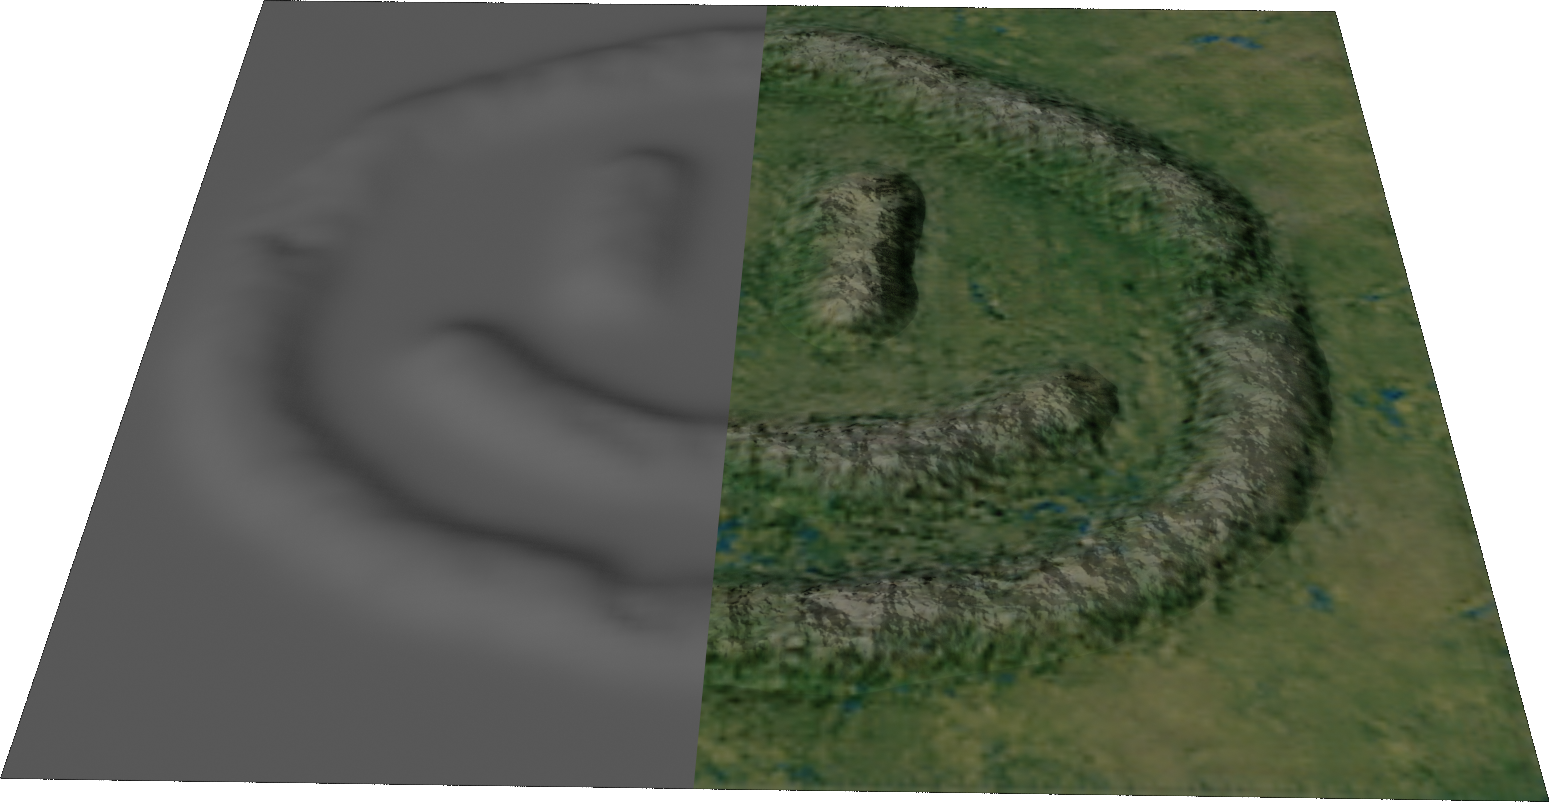
\includegraphics{other_images/smiley_heightmap_comparison_flat.png}
%     \label{fig:introduction_shading-comparison}
%     \caption{The application of shading (texturing and noise normal map) is an efficient method to whitewash any artifact in the original geometry of the terrain, faking a high resolution model, and hiding the unatural aspect of a synthetic model, improving artificially the realism of the terrain generation. Moreover, depending on the method used, the execution time of the aesthetic components generation may be longer than the geometry generation by order of magnitudes. Here, we trained a neural network (identical as the cGAN presented in \cref{sec:coral-island_cGAN}) to generate aerial images from elevation maps. Our synthetic height field represent a simple smiley (left) on which we applied the texture provided by the neural network and added fractal noise on the surface to add roughness to the material (right). }
% \end{figure}


% \subsubsection{Regeneration}
% The regeneration of procedurally generated models is an issue often overlooked. As the user is almost satisfied with its generation, he may decide to adjust slightly the parameters used. The challenges of the regeneration are multiple: How to let the user explore the \gloss{ParamSpace} of the model freely? How to ensure that a small change in a parameter induce a small change in the result? How to handle the edition from direct manipulations after regeneration? Those question arise directly from the realism-speed-control balance of our procedural models.

% Users can manually start the regeneration process to refresh or update a model. This allows the content to reflect new parameters or conditions as specified by the user. The generation speed has a strong influence on the possibility for the user to fine tune parameters as algorithms that can be executed in real-time or interactive-time keep the user active in his work. Longer execution times force him to find optimal parameters beforehand in order to create a satisfying model faster than if it was hand-made, which, when the model is not completely explicit, may feel impossible. 

% The fine-tuning speed can be improved by different strategies:
% \begin{Itemize}
%     \Item{} Modifications that have a local incidence on the resulting model requires only a local regeneration of the output. Limiting the spatial scope of an interaction is an efficient mean to keep at the same time a way to explore the \gloss{ParamSpace} of the algorithm while keeping the predictability of the outcome by avoiding global changes from a local edition.
%     \Item{} Live preview of the outcome can be displayed in a coarse computation, allowing to have a rough idea of the result without the full computation. This strategy is easier to develop with algorithms using refinement paradigms.
% \end{Itemize}

% [TODO]
% Interface controls: various tools and options in the user interface enable users to initiate regeneration. 
% This may include buttons or commands designed to reload or update the generated content based on user inputs.

% Customizable parameters: \\
% Adjustment of variables: before initiating regeneration, users can adjust parameters or settings to influence the outcome. 
% This might involve changing terrain features, texture types, or simulation conditions to achieve the desired results. \\
% Preview and validation: offering preview modes or validation checks helps users understand potential outcomes before finalizing the regeneration. 
% This feature ensures that users can visualize changes and make adjustments as needed.

% Issues with regeneration \\
% What to regenerate: \\
% Selective regeneration: deciding whether to regenerate the entire model or only specific parts is crucial. 
% For example, users may choose to regenerate just the terrain features while leaving other elements intact to preserve consistency. \\
% Scope and scale: determining how extensive the regeneration should be is essential. 
% This could involve minor updates or a complete overhaul of the generated content, depending on the changes required.

% How to regenerate: \\
% Algorithmic approaches: various methods can be used for regeneration, including reapplying existing algorithms or introducing new procedural rules. 
% These methods alter or update the existing content based on user inputs or new conditions. \\

% Incremental vs. complete regeneration: \\
% Incremental: gradual updates or changes applied to only parts of the generated content to minimize disruption and maintain consistency. \\
% Complete: full regeneration from scratch may be necessary for significant changes or when previous results are no longer valid, ensuring a fresh start if needed.

% \subsubsection{Interaction mechanisms}
% Interaction mechanisms are tools and methods used to facilitate user interaction with procedural generation: \\
% Parameter adjustment: user interfaces like sliders and controls enable adjustments to parameters such as terrain height or texture type. 
% Real-time feedback ensures users see the immediate impact of their adjustments. \\
% Guided creation: templates and presets offer predefined starting points that users can modify. 
% Assistive tools or wizards help guide users through the generation process, making it easier to understand and control the outcome. \\
% Direct manipulation: interactive tools allow users to directly manipulate generated content, such as sculpting terrain or painting textures. 
% Live updates reflect changes in real-time, facilitating immediate validation and adjustment.

% \subsubsection{Challenges and considerations}
% Challenges and considerations include balancing complexity and usability to ensure that sophisticated procedural systems remain user-friendly. \\
% Performance impact is another concern, especially in real-time applications where frequent updates are required. 
% Effective feedback and iteration mechanisms are crucial for helping users understand the impact of their interactions and refine their designs.

% Problems with user interactions \\
% Consistency: ensuring that regeneration maintains or enhances the consistency and quality of generated content is vital. 
% This involves avoiding artifacts or inconsistencies that could impact the user experience or the realism of the content. \\
% Feedback handling: effectively managing user feedback and requests for regeneration, which can vary in scope and detail, is important.
% Providing clear feedback mechanisms helps users understand how their inputs affect the generation process. \\
% Performance: addressing performance implications is crucial, particularly in real-time or interactive applications where frequent updates are necessary.
% Efficiently handling resource usage and computational demands during regeneration is key to maintaining a smooth experience.

% Action Storage
% Storage Formats:

% JSON: JavaScript Object Notation (JSON) files can be used to store regeneration actions and parameters. JSON is flexible and readable, making it a suitable format for saving and retrieving procedural settings.
% Other Formats: Alternatives such as XML, binary files, or custom formats may be used depending on specific needs or systems.
% Tracking Changes:

% Action History: Maintaining a history of user actions and regeneration events allows users to revert to previous states or track changes over time. This feature supports iterative development and refinement of generated content.
% Versioning: Implementing version control for procedural generation settings helps manage different versions of generated content, allowing users to compare and manage variations effectively.
% Restoration and Undo:

% Undo Mechanisms: Providing options for users to undo recent regeneration actions or revert to previous states enhances flexibility and control. This allows users to correct mistakes or adjust their approach as needed.
% Restoration of Defaults: Allowing users to restore default settings or regeneration conditions if custom changes lead to unsatisfactory results ensures that users can revert to a baseline if needed.
% Implementation Considerations
% Efficiency: Designing algorithms and systems to handle regeneration efficiently is crucial. This involves minimizing computational overhead and ensuring that updates are responsive and timely.

% User Experience: Creating intuitive interfaces and feedback mechanisms facilitates smooth user interactions with the regeneration process. Ensuring that users can easily understand and control the regeneration helps improve their overall experience.

% Error Handling: Implementing robust error handling and recovery mechanisms addresses potential issues that may arise during regeneration, such as unexpected results or system failures. Effective error management ensures that users can continue working without significant disruptions.



% \section{Procedural biogeocoenosis generation}
% Bla bla bla, terrain + atmosphere = environment, environment + living beings = biogeocoenosis bla bla 

% \subsection{}

% \subsection{Fluid simulations}
% Fluid simulations are an essential component of procedural terrain generation, particularly for modeling the behavior of water and its interactions with the terrain. These simulations are crucial for creating realistic and dynamic environmental models that accurately reflect natural phenomena, such as river flow, coastal erosion, sediment transport, and overall hydrology.

% At the core of fluid simulations are the Navier-Stokes equations, which describe the motion of fluid substances. These equations account for various forces acting on a fluid, such as pressure, viscosity, and external forces like gravity. 
% \begin{align}
%     \rho \left( \frac{\partial \mathbf{u}}{\partial t} + (\mathbf{u} \cdot \nabla) \mathbf{u} \right) = -\nabla p + \mu \nabla^2 \mathbf{u} + \mathbf{f}
% \end{align}
% Where $\mathbf{u} = (u, v, w)$ is the fluid velocity vector, with components $u$, $v$, and $w$ in the $x$-, $y$-, and $z$-directions, respectively, $t$ is time, $\rho$ is the fluid density, $p$ is the pressure field within the fluid, $\mu$ is the dynamic viscosity of the fluid, $\nabla p$ is the pressure gradient force, $\mu \nabla^2 \mathbf{u}$ is the viscous diffusion term, representing the effects of internal friction within the fluid and finally, $\mathbf{f}$ represents external body forces, such as gravity.

% For an incompressible fluid like water, the Navier-Stokes equations can be simplified by assuming that the fluid density remains constant, leading to the incompressibility condition:

% \begin{align}
%     \nabla \cdot \mathbf{u} = 0
% \end{align}

% This condition ensures that the volume of fluid elements remains unchanged as they move through space, which is crucial for accurately simulating water flow.

% The Navier-Stokes equations are highly non-linear, which means that even small changes in the input conditions can lead to significant and unpredictable changes in the fluid's behavior. The non-linearity makes solving these equations a expensive computational problem, as it requires iterative methods to find stable solutions. Each step of the simulation must balance the forces acting on the fluid, such as pressure and viscosity, while ensuring that the solution remains physically accurate and stable over time. This process becomes particularly demanding when aiming for realistic, high-resolution simulations where fine details like turbulence and surface tension must be accurately captured.In this case we require dense computational grids or a large number of particles, and these elements must be updated frequently to maintain the realism of the simulation, which exponentially increase the computations and the memory used.

% The computation cost is further amplified when simulations are performed in 3D space. Unlike 2D simulations, where calculations are confined to a plane, 3D simulations must account for the full complexity of fluid movement in all directions. This increases the number of computations required, making real-time applications like as video games and interactive simulations almost incapable to use them.

% Different fluid solvers have been developed to approximate the solutions to the Navier-Stokes equations, each with its strengths and weaknesses. These solvers vary in how they represent the fluid (the Lagrangian approach using particles or the Eulerian approach with discrete grids, or a combination of both) and how they handle the computational trade-offs between accuracy, stability, and performance. The choice of a fluid solver depends on the specific requirements of the simulation, such as the need for real-time performance, the level of detail required, or the types of fluid behavior being modeled.

% \subsubsection{Marker-And-Cell (MAC) Method}

% The Marker-And-Cell (MAC) method is one of the earliest and most fundamental grid-based techniques for simulating incompressible fluid flows. In the MAC method, the fluid's velocity components are stored at the faces of grid cells, while pressure values are stored at the cell centers. Marker particles are used to track the fluid's free surface, ensuring that fluid interfaces and boundaries are accurately captured. The MAC method excels at maintaining the incompressibility condition of fluids and accurately modeling pressure fields, which are important for realistic fluid dynamics. Because of its emphasis on accuracy and detailed pressure modeling, MAC is more oriented toward realism, especially in scenarios where the precise behavior of fluids is essential. However, its grid-based nature can lead to challenges in handling complex geometries and fine details at fluid boundaries, as the resolution is limited by the grid size. Moreover, the method can be computationally intensive, especially for high-resolution grids, making it less ideal for real-time applications.

% \subsubsection{Stable Fluids}

% Building on the grid-based approach of the MAC method, the Stable Fluids method addresses key stability issues that arise in fluid simulations \cite{Stam1999}. Stable Fluids uses a semi-Lagrangian advection scheme and implicit solvers to achieve stability even with large time steps, which is particularly advantageous in real-time applications like video games or interactive simulations. This method is designed with performance in mind, allowing for the simulation of fluid motion without the numerical dissipation that can degrade the accuracy of results over time, which was a common problem in other grid-based methods. While Stable Fluids prioritize performance and stability, particularly in real-time environments, the use of implicit solvers can introduce smoothing effects that reduce the sharpness of fine details in the fluid's motion. Additionally, the method's reliance on grid resolution still limits its ability to represent highly detailed surface interactions, making it a good compromise between realism and performance.

% \subsubsection{Particle-In-Cell (PIC) Method}

% The Particle-In-Cell (PIC) method represents a hybrid approach that combines the strengths of particle-based and grid-based methods. Fluid properties are stored on a grid, but the fluid's motion is tracked using particles, which carry velocity and position information only. The particles interact with the grid to update the fluid's velocity field, and the grid provides a stable mean for solving the fluid dynamics equations. PIC is particularly useful for capturing the large-scale motion of fluids, benefiting from the grid's stability while using particles to track detailed fluid behavior. However, the method leans more toward performance over accuracy due to its hybrid nature and ability to handle large-scale fluid movements efficiently. A major downside of PIC is its tendency toward numerical dissipation, where the fluid's kinetic energy is artificially reduced over time, leading to a loss of fine details, especially in turbulent flows. This dissipation occurs because the interpolation between particles and the grid tends to average out small-scale variations in velocity, making PIC less suitable for scenarios where high fidelity and detail are required.

% \subsubsection{Fluid-Implicit Particle (FLIP) Method}

% The Fluid-Implicit Particle (FLIP) method is an evolution of the PIC method designed to address its numerical dissipation problem \cite{Brackbill1988}. FLIP retains the grid-particle hybrid approach but modifies how particle velocities are updated. Instead of fully relying on the grid's velocity field, FLIP updates particle velocities by applying only the changes in the grid's velocity field, preserving the fluid's kinetic energy and maintaining the detail in small-scale motions. This approach significantly reduces numerical dissipation, making FLIP more oriented toward realism, particularly in simulations that require detailed fluid dynamics like splashing, swirling, and other turbulent effects. However, FLIP is more computationally expensive than PIC and can suffer from instability issues, particularly when dealing with highly turbulent flows. The increased computational cost and the need for careful tuning of simulation parameters to maintain stability make FLIP less ideal for performance-focused applications but suitable for scenarios where high fidelity and detailed fluid behavior are essential.

% \subsubsection{Smoothed Particle Hydrodynamics (SPH)}

% Smoothed Particle Hydrodynamics (SPH) \cite{Muller2003} is a purely particle-based method that models fluids using discrete particles, each representing a small volume of fluid. These particles interact with each other based on smoothing kernels, which define the influence of one particle on its neighbors over a certain distance \cite{Koschier2022}. SPH is particularly well-suited for simulating free-surface flows, such as waves, splashes, and other fluid phenomena where the interaction between fluid particles is complex and highly dynamic. Due to its ability to handle complex boundaries and fluid interfaces naturally, SPH is much more focused on realism, especially in scenarios that require accurate computation of fluid dynamics and interactions. However, SPH is computationally intensive, especially for high-resolution simulations where a large number of particles is required. Additionally, SPH can suffer from stability issues, such as particle clumping or excessive smoothing, which can detract from the realism of the simulation if not carefully managed. These factors make SPH better suited for applications where realism is prioritized over performance, particularly in high-fidelity simulations used in film and scientific research, but not for real-time applications.

% We can find improvements \cite{Roose2011}, can represent may elements \cite{Iwasaki2010}, either fluid or sediments \cite{Lenaerts2009}, so it is often used to simulate accurately water bodies \cite{Nikeghabali2018}.

% Some other models exist, and are often proposed in OpenFOAM, either using grids, or particles, or an hybrid version \cite{Caretto1973} [ADD OTHER REFERENCES]. But some works tend in directions that are more "procedural" like the use of cellular automata \cite{Boldea2009,Cattaneo2005}, while other toward a more modern approach with the use of deep learning \cite{Tompson2017} [ADD OTHER REFERENCES].






% \subsection{Fluid simulations}

% Fluid simulations are almost inevitable in representing natural phenomena in terrain generation, particularly in modeling water flow, erosion, and sediment transport. These simulations are used for creating realistic and dynamic environmental models that accurately reflect the interactions between fluids and terrain. The ability to simulate fluid behaviors such as river currents, coastal erosion, and sediment deposition is fundamental to producing realistic terrains.

% Fluid simulations can be categorized into various methods, each with its unique applications. Techniques like Particle-In-Cell (PIC), Fluid-Implicit Particle (FLIP), and Stable Fluids are commonly used to simulate fluid dynamics. PIC combines particles with a grid to offer a straightforward approach for basic fluid simulations and visualizations. FLIP builds on the PIC method by enhancing accuracy and efficiency through a hybrid approach that merges particle and grid techniques, making it suitable for complex fluid behaviors. Stable Fluids, a grid-based method, is designed for simulating stable, incompressible fluids with minimal computational complexity, often used in interactive applications where real-time rendering is required.

% More sophisticated methods include Smoothed Particle Hydrodynamics (SPH) and Marker-And-Cell (MAC). SPH is a particle-based method where fluid properties are represented by particles that interact based on smoothing kernels, useful for detailed simulations, including interactions between fluids and terrain. MAC and other grid-based approaches use a grid to simulate fluid behavior, providing detailed and accurate representations suitable for various scales of environments. Hybrid methods combine the strengths of grid and particle approaches, balancing the need for detail with performance requirements in complex simulations.

% Fluid simulations are integral to terrain generation, particularly in modeling erosion and sediment transport. These simulations allow for the realistic modeling of erosion processes, which affect terrain features like riverbeds and valleys over time. By simulating how fluids interact with the terrain, these models can show how sediment is moved and deposited, contributing to the natural evolution of the landscape. Water flow and hydrology are other applications of fluid simulations in terrain generation. Simulating surface water dynamics, such as the flow of rivers, lakes, and wetlands, helps create realistic environments where water interacts dynamically with the terrain. 
% % Additionally, subsurface flow simulations model groundwater movement and its interactions with surface features, adding another layer of realism to the terrain.

% % In interactive environments, such as video games and virtual simulations, real-time fluid simulations are crucial for creating dynamic water interactions. These simulations enable the depiction of responsive and changing environments, where water flow can be influenced by user actions or environmental conditions, enhancing the immersive experience.

% While significant for terrain generation, fluid simulations still present important challenges. The main issue is the computational resources required to run accurate and detailed simulations. Performance trade-offs are often necessary, especially in real-time applications where the simulation must balance accuracy with computational efficiency. Complex 2D (or 2.5D) fluid simulations already require powerful hardware, including advanced processors and substantial memory, to handle the intensive calculations involved. 3D simulations are even more computationally expensive, as the third dimension has to be taken into account.

% Another challenge lies in balancing accuracy with realism. While detailed fluid dynamics can produce highly realistic simulations, they often come at the cost of performance. Simulation artifacts, or inaccuracies, can also impact the perceived realism of the terrain, requiring careful attention to detail in the modeling process. Integrating fluid simulations with terrain models presents its own set of challenges. Ensuring that fluids interact seamlessly with the terrain, such as through fluid erosion or sediment deposition, requires sophisticated techniques to maintain consistency between the simulated fluid behaviors and the terrain features.

% Recent developments in fluid simulation technology have focused on enhancing both the accuracy and efficiency of these simulations. Advancements in algorithms have led to new techniques that improve the realism and computational performance of fluid models. There has also been significant progress in real-time fluid simulation, with innovations aimed at improving interactivity.

% The integration of Deep Learning and Machine Learning into fluid simulations represents a recent trend in this field. AI-enhanced simulations use machine learning to refine fluid simulation accuracy and adaptivity, enabling more realistic and responsive environments. Predictive models, powered by AI, can simulate complex fluid behaviors based on historical data, offering new possibilities for dynamic and evolving terrain representations.



% - Definition and purpose: \\
% ** Overview: explanation of fluid simulations and their role in representing natural phenomena in terrains, including water flow, erosion, and sediment transport. \\
% ** Importance: impact of accurate fluid simulations on creating realistic terrain and environmental models.\\
% \subsection{Types of fluid simulations}
% - 2D fluid simulations: \\
% ** Particle-In-Cell (PIC): \\
% *** Concept: combines particles with a grid to simulate fluid dynamics. \\
% *** Applications: used for simpler simulations and visualizations. \\
% ** Fluid-Implicit Particle (FLIP): \\
% *** Concept: a hybrid method that combines particle and grid approaches for better accuracy and efficiency. \\
% *** Applications: suitable for capturing complex fluid behaviors in 2D environments. \\
% ** Stable Fluids: \\
% *** Concept: a grid-based method for simulating stable, incompressible fluids with less computational complexity. \\
% *** Applications: often used in interactive applications where real-time performance is crucial.\\
% - 3D fluid simulations: \\
% ** Smoothed Particle Hydrodynamics (SPH): \\
% *** Concept: a particle-based method where fluid properties are represented by particles that interact based on smoothing kernels. \\
% *** Applications: useful for highly detailed simulations of fluids, including interactions with terrain. \\
% ** Grid-based methods: \\
% *** Concept: methods like Marker-And-Cell (MAC) and Navier-Stokes equations applied on a grid to simulate fluid behavior. \\
% *** Applications: used for detailed and accurate 3D simulations, including large-scale environments. \\
% ** Hybrid methods: \\
% *** Concept: combining grid and particle approaches to leverage the strengths of both methods.\\
% *** Applications: balancing detail and performance in complex simulations. 

% \subsection{Applications in terrain representation}
% - Erosion and sediment transport: \\
% ** Simulation of erosion: how fluid simulations model erosion processes affecting terrain features such as riverbeds and coastlines. \\
% ** Sediment movement: modeling the transport and deposition of sediment, contributing to realistic terrain evolution. \\
% - Water flow and hydrology: \\
% ** Surface water dynamics: representing the flow of water across terrain surfaces, including rivers, lakes, and wetlands. \\
% ** Subsurface flow: simulating groundwater movement and interactions with terrain features. \\
% - Interactive environments: \\
% ** Real-time simulations: implementing fluid simulations in interactive applications, such as video games and virtual environments, where dynamic water interactions are crucial. 

% \subsection{Challenges and considerations}
% - Computational resources: \\
% ** Performance trade-offs: balancing simulation accuracy with computational efficiency, especially for real-time applications. \\
% ** Hardware requirements: the need for powerful processors and memory to handle complex 3D fluid simulations. \\
% - Accuracy vs. realism: \\
% ** Detail vs. performance: finding the right balance between detailed fluid dynamics and the practical limitations of simulation resources. \\
% ** Simulation artifacts: addressing potential artifacts or inaccuracies in simulations that can impact realism. \\
% - Integration with terrain models: \\
% ** Interaction with terrain: ensuring fluid simulations integrate seamlessly with terrain models, including handling interactions such as fluid erosion or deposition. \\
% ** Data consistency: maintaining consistency between simulated fluid behaviors and terrain features for accurate representations. 

% \subsection{Recent developments and future trends}
% - Advancements in algorithms: \\
% ** New techniques: emerging algorithms and methods that enhance the accuracy and efficiency of fluid simulations. \\
% ** Real-time improvements: innovations aimed at improving real-time performance and interactivity in fluid simulations. \\
% - Integration with Deep Learning and Machine Learning: \\
% ** AI-enhanced simulations: using machine learning to improve fluid simulation accuracy and adaptivity. \\
% ** Predictive models: leveraging AI to predict and simulate complex fluid behaviors based on historical data. 

% - Very important in procedural terrain generation \\
% - Allows justifying the geophysics of a simulation/generation \\
% - Quite fast solutions in 2D (PIC, FLIP, Stable Fluids, SPH, etc.) \\
% - But becomes much heavier and memory-intensive in 3D \\
% - ...

% \subsection{Vegetation generation}
% Bla bla...






\section{Underwater landscapes}
- Use "seascape" instead of "landscape" and "aerial landscapes" for above water. \\
** Not official terms, but may be very useful for the rest of this thesis..! \\
- Describe main differences with landscape generation \\
- Describe coral reef islands ecosystems.

\subsection{Main differences with aerial terrains}
In the field of terrain generation, particularly when it comes to modeling underwater landscapes, the challenge is to accurately represent complex environments that include both geological and biological features. The underwater world is filled with diverse structures, ranging from vast coral reefs to intricate cave systems, each requiring specialized techniques to model their unique characteristics.

\subsubsection{3D Data for underwater landscapes}

One of the most challenging aspects of underwater landscape modeling is capturing the complexity of its structure. Taking the example of coral reefs,these environments feature highly intricate 3D structures, including branching corals, coral mounds, and encrusting forms. These formations are not just surface-level features; they extend into the terrain with voids and cavities, such as caves, grottos, and karst networks, which add layers of complexity to their representation. Accurate modeling of coral reefs demands that the porous and irregular nature of these formations is represented in high detail, which is a significant challenge due to the variability of their structures.

In addition to biological features, underwater landscapes are shaped by geological processes that must also be accurately represented. For example, sedimentary layers and underwater geological formations like seamounts and ridges are important components of the terrain. 
% Furthermore, volcanic activity, including underwater volcanos and hydrothermal vents, significantly impacts the landscape and ecosystem, necessitating their inclusion in any comprehensive model of underwater environments.

To gather the data needed for such detailed modeling, advanced measurement techniques are employed. Sonar, including multi-beam echo sounders, and LIDAR (Light Detection and Ranging) are commonly used to capture detailed 3D data of underwater terrains. These technologies allow for the mapping of areas that are otherwise difficult to access, providing the foundational data necessary for accurate terrain generation. Remote sensing technologies also play a major role, enabling the collection of data over large and remote areas, further enhancing the model's accuracy, but represent a significant challenge as the approvision of humans and hardware in these areas is far from easy to achieve.

\subsubsection{Interdisciplinary data integration}

Accurately modeling underwater landscapes requires more than just geological data; it necessitates an interdisciplinary approach that integrates biological and ecological data. Geological validation is an important step in this process, involving collaboration with geologists and marine scientists to ensure that the models are not only scientifically accurate but also reflective of real-world conditions. This validation process ensures that the generated models accurately depict the geological and biological features present in underwater environments.

Biological data is also essential, particularly when modeling coral reefs and other marine ecosystems. Incorporating data on coral species, marine biodiversity, and ecosystem dynamics allows for the creation of realistic and biologically accurate representations. Additionally, the impact of biological processes, such as coral growth patterns and marine erosion, must be considered, as these factors significantly influence the terrain shape over time.

However, one of the major challenges in modeling underwater landscapes is the scarcity of high-resolution data, especially in remote, protected or less studied areas. This data scarcity makes it difficult to create detailed and accurate models. Another challenge lies in the integration of diverse data types, geological, biological, hydrological, etc, into a cohesive and comprehensive model. Effective integration requires complex techniques to ensure that all aspects of the underwater environment are accurately represented.

\subsubsection{Multi-scale modeling}

Underwater landscapes are characterized by features that vary greatly in scale, from vast underwater mountains and ridges to small-scale elements like individual coral polyps and marine vegetation. This diversity in scale necessitates multi-scale modeling techniques that can accommodate both large and small features within the same model.

\citep{ParisThesis} classified the different geological structures in four different spatial scales: the \textit{megascale} describes landforms spread on more than \si{100}{km} such as continents or mountain ranges, the \textit{macroscale} between \si{1}{km} and \si{100}{km} like river or cave networks, the \textit{mesoscale} ranging from \si{10}{m} to \si{1}{km} contains most complex structures (arches, ravines, cliffs, ...) and finally the \textit{microscale} for features between \si{10}{cm} and \si{10}{m}, like sand ripples, ventifacts, rocks, etc. Generally, we consider as \textit{large-scale} features that can be seen from far away and \textit{small-scale} elements for which somebody has to be to close to to observe it.

Large-scale features, such as underwater mountains and ridges, define the macrostructure of the landscape. These must be integrated seamlessly with small-scale features, such as detailed sedimentary textures and small coral formations, to ensure that the terrain is represented accurately across different scales.

[TODO]

% One of the key techniques used in multi-scale modeling is \gloss{LOD}, which involves adjusting the level of detail in the model based on factors like user interaction or viewing distance. Adaptive LOD techniques help balance the need for visual fidelity with the performance demands of rendering complex terrains. The goal is to preserve detail across scales, ensuring that both macro and micro features are represented without losing important details when the model is scaled or zoomed.

% Visualization techniques also play a crucial role in representing underwater landscapes accurately. Hydrographic mapping is one such technique, providing specialized methods to visualize underwater features clearly. Additionally, the use of textures and lighting that simulate underwater conditions, such as light absorption and scattering, enhances the realism of the model. These techniques help create visually accurate and scientifically meaningful representations of underwater environments.

The procedural generation of underwater landscapes involves the integration of advanced 3D data collection techniques, interdisciplinary collaboration, and multi-scale modeling approaches. Modeling underwater environments, from the complex structures of coral reefs to the accurate representation of geological and biological features, requires innovative solutions that combine geological plausibility with visual realism.


% - 3D data: \\
% ** Coral landscapes: addressing challenges in modeling coral reefs and underwater features. \\
% ** Cavities: representing underwater caves and karst formations. \\
% - Interdisciplinary data: \\
% ** Geological validation: integrating expert knowledge for accurate modeling. \\
% ** Challenges: fewer experts and more uncertainties in underwater environments. \\
% ** Data scarcity: limited data availability for detailed underwater landscapes. \\
% - Need for multi-scale: \\
% ** Integration of large and small elements. \\
% ** Level of Detail (LOD): Techniques for managing detail across different scales.

% \subsubsection{3D data}
% - Coral landscapes: \\
% ** Complex structures: coral reefs feature complex 3D structures with intricate patterns including branching corals, coral mounds, and encrusting forms. These structures often have a high degree of variability and detail. \\
% ** Void spaces: coral reefs contain many voids and cavities such as caves, grottos, and karst networks, adding to the complexity of modeling these environments. \\
% ** Challenges: modeling coral reefs requires accurately representing the porous and irregular nature of coral formations, which can be challenging due to the high level of detail and variability. \\
% - Geological features: \\
% ** Sedimentary layers: representing sedimentary layers and underwater geological formations such as seamounts and underwater ridges. \\
% ** Volcanic activity: incorporating features such as underwater volcanos and hydrothermal vents, which affect the landscape and ecosystem. \\
% - Measurement and data collection: \\
% ** Sonar and LIDAR: using sonar (e.g., multi-beam echo sounders) and LIDAR (Light Detection and Ranging) to collect detailed 3D data of underwater terrain. \\
% ** Remote sensing: utilizing remote sensing technologies to map and model underwater landscapes, especially in areas that are difficult to access.

% \subsubsection{Interdisciplinary data}
% - Geological validation: \\
% ** Expert consultation: collaborating with geologists and marine scientists to validate and refine models based on real-world observations and data. \\
% ** Data accuracy: ensuring that the generated models accurately reflect real underwater geological and biological features. \\
% - Biological data: \\
% ** Coral and marine life: integrating data on coral species, marine biodiversity, and ecosystem dynamics to create realistic and biologically accurate representations. \\
% ** Ecological impact: considering the impact of various biological factors on the terrain, such as coral growth patterns and marine erosion. \\
% - Challenges: \\
% ** Data scarcity: limited availability of high-resolution data for some underwater environments, especially in less studied or remote areas. \\
% ** Integration: combining geological, biological, and hydrological data effectively to create comprehensive and accurate models. 

% \subsubsection{Multi-scale modeling}
% - Large vs. small scale elements: \\
% ** Macro features: incorporating large-scale features such as underwater mountains, ridges, and large coral formations. \\
% ** Micro features: modeling small-scale elements such as individual coral polyps, marine vegetation, and detailed sedimentary textures. \\
% - \Gloss{LOD} (LOD): \\
% ** Adaptive LOD: using techniques to adjust the level of detail based on user interaction or view distance to balance performance and visual fidelity. \\
% ** Detail preservation: ensuring that both macro and micro-scale features are accurately represented without losing important details during scaling or zooming. \\
% - Visualization techniques: \\
% ** Hydrographic mapping: employing specialized visualization techniques to represent underwater features clearly and accurately. \\
% ** Texture and lighting: using textures and lighting models that simulate underwater conditions, such as light absorption and scattering in water.

% - 3D Data \\
% ** Coral landscapes filled with voids \\
% ** Many cavities (caves, grottos, karst networks) \\
% - Interdisciplinary Data \\
% ** Rather common with terrain generation \\
% ** => Geological validation with experts \\
% ** For underwater, \\
% *** Fewer experts, \\
% *** More uncertainties \\
% *** Based more on observations \\
% *** Few data (coral landscapes < 0.1\% of oceans), for significant biological impact (25\% marine biodiversity) \\
% ** Mix of geology, biology, hydrology, and physics (especially fluid dynamics) \\
% - Need for multi-scale \\
% ** Not limited to underwater \\
% ** Integrate large elements (mountains) with small elements (vegetation) \\
% ** LOD \\
% - ...

\subsection{Coral biology}
\label{sec:state-of-the-art_biology}

Coral reefs have intrigued humans for centuries, with early observations by ancient civilizations often misunderstanding these structures as mysterious sea plants or rocks. The study of coral reefs gained scientific momentum during the era of exploration, particularly through the work of figures like Captain James Cook and Charles Darwin. Darwin's theory of atoll formation, developed during his voyage on the HMS Beagle, was a significant milestone, proposing that atolls form around sinking volcanic islands as coral growth keeps pace with subsidence.

The 20th century brought technological advancements, such as scuba diving and sonar, which allowed scientists to directly observe and map coral reefs, deepening our understanding of their biology and ecological significance. In recent decades, tools like remote sensing and genetic analysis have further expanded our knowledge, highlighting the critical role of coral reefs in marine biodiversity and their vulnerability to environmental changes.

\subsubsection{Anatomy of coral reefs}

\subsubsubsection{Coral polyps}

Coral polyps are the essential building blocks of coral reefs. These tiny, soft-bodied organisms, just a few millimeters in diameter, form the vast structures of coral reefs. Each polyp consists of a sac-like body with a central mouth surrounded by tentacles equipped with stinging cells (nematocysts) for defense and capturing prey.

The body of the polyp is anchored to a hard surface, which it helps create by secreting calcium carbonate \ch{CaCO3}. This secretion forms a protective exoskeleton around the polyp, allowing it to attach securely to the substrate or to other polyps in a colony. This secretion process creates the coral's hard structure, which becomes the foundation of the reef.

Reproduction in coral polyps occurs in two main ways: asexual and sexual reproduction. Asexually, polyps reproduce through a process called budding, where new polyps form from the sides of an existing polyp. These new polyps remain attached, leading to the growth of a larger coral colony. In sexual reproduction, polyps release eggs and sperm into the water during spawning events, where fertilization occurs externally. The resulting larvae settle onto a suitable substrate, developing into new polyps and eventually forming new colonies.

Coral polyps are in a symbiotic relationship with zooxanthellae, a type of photosynthetic algae that live within the tissues of the coral polyps, providing them with vital energy through photosynthesis, fueling its growth and calcification.

In return, the coral provides the zooxanthellae with protection and access to sunlight. This mutualistic relationship is highly efficient, allowing corals to thrive in the nutrient-poor waters of tropical oceans.

However, this relationship is fragile. When corals are exposed to environmental stressors such as elevated water temperatures, they may expel their zooxanthellae in a phenomenon known as coral bleaching. Without the algae, the coral loses its primary energy source, leading to a whitening of the coral and, if conditions do not improve in the next weeks, eventual death.

\subsubsubsection{Coral colonies}
Coral polyps, though individually small and simple, have the remarkable ability to form large, complex colonies that create the structure of coral reefs. These colonies exhibit a variety of growth patterns, each of which plays a different role in the overall architecture and ecological function of coral reefs.

Once established, coral colonies can develop into a wide range of growth forms, each adapted to specific environmental conditions and with unique functions to contribute to the reef shape.

Massive corals, like those in the genus \textit{Porites}, grow in boulder-like forms. They tend to grow more slowly than other types but are much more resistant to physical damage from waves and storms. They contribute to the long-term stability and resilience of coral reefs. Massive corals can live for hundreds of years, with some colonies growing to several meters in diameter. Their dense, solid structure provides a stable and enduring foundation for the reef, making them useful for the long-term stability of the reef ecosystem. Their robust skeletons can withstand strong wave action, storms, and other environmental stresses that would easily damage more delicate coral types. As they grow and expand, massive corals create the core of the reef, providing a solid base that other corals and marine organisms can build upon. Their presence is vital for maintaining the reef's overall integrity and resilience.

In contrast, branching corals, such as those in the genus \textit{Acropora} (e.g., staghorn corals), look like a tree structure with numerous branches. These corals grow rapidly, extending outward to maximize exposure to sunlight. The dense thickets formed by branching corals provide essential habitat for a wide variety of marine species, from small fish to invertebrates. This growth form is particularly present in shallow, well-lit waters where competition for space and light is intense. This rapid growth allows them to quickly occupy space and expand the reef's surface area. The three-dimensional architecture of branching corals provides important habitats for a variety of marine life, including small fish and invertebrates, offering them protection from predators and strong currents. However, branching corals are relatively fragile and can be easily damaged by storms, waves, or human activity. Their ability to regenerate through fragmentation allows them to recover quickly from physical damage, but they do not contribute significantly to the reef's overall structural strength.

Similarly, foliose corals like in the genus \textit{Astreopora}, which form leaf-like structures, add another dimension to reef complexity. These corals grow in overlapping layers, creating sheltered environments within the reef that are ideal for smaller marine organisms. Foliose corals can be particularly abundant in areas with moderate water movement, where their shape helps capture food particles from the water.

Corals that grow in flat, horizontal formations are known as table corals or plate coral, such as \textit{Acropora}, can spread out to cover large areas, creating expansive, flat surfaces that provide important habitats for animals and other coral colonies. Their growth form allows them to efficiently capture sunlight, making them well-suited for shallow reef environments.

Some corals, known as encrusting corals like in the genus \textit{Cyphastrea}, grow as a thin layer over hard substrates, including rocks, dead coral skeletons, and other surfaces. They are particularly adept at covering large areas of the reef, often outcompeting other organisms for space. Their growth form helps to bind loose sediments and rubble together, contributing to the stabilization of the reef's foundation. Although encrusting corals do not add significant height or volume to the reef, they are critical for cementing the reef structure, preventing erosion, and enhancing the overall stability of the reef. By filling in gaps between other coral colonies and consolidating the reef framework, encrusting corals help maintain the reef's structural cohesion, which is essential for its longevity.

The position of different coral types within the reef varies depending on factors such as water depth, wave exposure, and light availability. Massive corals are typically found on the reef slope, where the water is deeper and more stable. Encrusting corals thrive in the less turbulent waters of the deep reef, where they can spread across stable surfaces. Branching corals, such as Acropora species, are often found on the reef crest and fore reef, where they are exposed to strong wave action and plenty of sunlight. Their fast growth and ability to regenerate quickly make them well-suited for these dynamic environments. Foliose corals are often found on the reef flat and in the back reef areas, where the water is calmer and light levels are moderate. Table corals are also commonly found in shallow reef environments, where they can maximize their exposure to sunlight.

These varied growth patterns not only shape the physical structure of coral reefs but also create habitats that support immense biodiversity, making coral reefs, even if representing less than 0.1\% of the ocean area, some of the most biologically diverse ecosystems on Earth, with about 25\% of the marine species.

\subsubsubsection{Reproduction}
The formation and expansion of coral colonies are driven by a combination of sexual and asexual reproductive strategies, each of which plays a vital role in the growth, survival and spread of coral species.

Asexual reproduction is the primary mechanism by which coral colonies expand and repair themselves. The most common form of asexual reproduction is budding, where new polyps are produced from the body of an existing polyp. These new polyps remain attached to the parent polyp, leading to the growth of a larger, stronger, interconnected colony. The shared calcium carbonate skeleton secreted by these polyps provides the structural foundation for the entire colony.

Another important method of asexual reproduction is fragmentation, in which parts of the coral break off, often due to physical disturbances such as storms or strong currents, emit fragments with polyps that can then reattach to a suitable substrate and form new colonies further away. Species like \textit{Acropora} spp. and \textit{Pocillopora} spp. are known for their ability to reproduce through fragmentation, making them proliferic in dynamic environments. Similarly, polyp bail-out, where individual polyps detach from the colony in response to environmental stress allows corals to survive adverse conditions and spread its colonies. Species such as \textit{Fungia} spp. and \textit{Scleractinia} spp. have been observed to reproduce through polyp bail-out.

Sexual reproduction is essential for generating new colonies and ensuring genetic diversity within coral populations. Many coral species, particularly those that are broadcast spawners, engage in mass spawning events. During these events, numerous corals simultaneously release eggs and sperm into the water column, where fertilization occurs externally. The resulting larvae (planulae), are carried by ocean currents, sometimes over great distances, before settling onto a suitable substrate where they can develop into new polyps and establish a new colony. The precise synchronization of these spawning events, while not fully understood, is thought to be influenced by environmental elements such as lunar cycles, water temperature, and daylight length. Species such as \textit{Acropora} spp. and \textit{Porites} spp. are typical broadcast spawners, relying on this strategy to disperse their offspring and colonize new areas of the reef.

Some coral species are brooders, where fertilization occurs internally within the polyp. The larvae are retained inside the polyp until they are more developed and ready to settle soon after being released. This strategy often results in the larvae settling near the parent colony, contributing to the growth of dense coral clusters. \textit{Pocillopora} spp. and \textit{Stylophora} spp. are examples of brooding corals that employ this strategy, leading to the formation of tightly clustered colonies that enhance the local complexity of the reef.

Together, these reproductive strategies ensure the survival, expansion, and genetic diversity of coral populations. They enable coral reefs to adapt to changing environmental conditions, recover from disturbances by colonizing new areas and reinforce existing structures.


\subsubsection{Corals, animals and vegetation interactions}

Coral reefs are dynamic ecosystems where corals, algae, and reef-dwelling animals are constantly interacting, with each playing a vital role in the health and stability of the reef. The competition between corals and algae is a fundamental aspect of these interactions. Both corals and algae compete for the same resources: sunlight, nutrients, and substrate. However, their growth strategies differ significantly. Corals are slow-growing, reef-building organisms that provide the structural foundation of the reef, while algae are generally fast-growing and can quickly colonize available space, especially when nutrient levels are elevated due to pollution or when populations of herbivores, such as fish and sea urchins, are reduced due to overfishing or diseases. This algal overgrowth can suffocate coral colonies, blocking sunlight and hindering coral growth and reproduction. A shift in the ecosystem from a coral-dominated system to an algal-dominated significantly reduces the structural complexity of the reef, as algae do not build the rigid frameworks that corals do. The loss of coral cover and the dominance of algae decrease the reef's ability to provide habitat for marine life, leading to a decline in biodiversity and altering the dynamics of the entire ecosystem.

In addition to controlling algae, certain reef animals contribute to coral health through bioerosion, a process where organisms like parrotfish and certain invertebrates break down dead coral structures, which help recycle calcium carbonate within the reef ecosystem. The fine sediment produced by bioerosion can fill in gaps between living coral colonies, stabilizing the reef and providing a more solid foundation for new coral growth. 

Fishes also contribute to coral preservation through nutrient cycling. As fishes move through the reef and excrete waste, they release nutrients that can be utilized by corals and other reef organisms. These nutrients can be absorbed by corals to grow, especially in nutrient-poor environments where external nutrient sources are limited. Furthermore, the physical presence of fish within the reef can enhance water circulation, which helps distribute nutrients and oxygen throughout the reef, supporting coral health and resilience.

Corals have evolved various defense mechanisms to protect themselves from algal overgrowth and other threats. Some corals produce chemical compounds that deter algal growth or attract herbivorous fish that feed on algae. Additionally, certain coral species engage in mutualistic relationships with small fish or invertebrates that help defend the coral from algal encroachment and predation.

Environmental changes, particularly those driven by climate change, can disrupt the balance between corals and algae. Warmer ocean temperatures and acidification by increased \ch{CO2} can increase the frequency and severity of coral bleaching events, weakening corals and giving algae a competitive advantage. Additionally, nutrient enrichment from agricultural runoff, sewage, and other sources can lead to algal domination on coral reefs. 

Fish and other marine organisms derive significant benefits from living in coral reef habitats, which are essential for their survival, growth, and reproduction. Coral reefs offer a complex three-dimensional structure that provides shelter and protection from predators, particularly for juvenile fish. This protective environment increases the chances of survival for many species.

Additionally, coral reefs serve as critical breeding and nursery grounds. The sheltered environments within the reef are ideal for spawning and raising young, offering protection to eggs and larvae. Coral reefs also facilitate important social interactions, such as territory establishment and mating behaviors, which are vital for reproduction and species survival.

Lastly, some fish species engage in mutualistic relationships with corals, such as clownfish with anemones, gaining protection while providing benefits like nutrient exchange or cleaning services. These interactions underscore the interdependence of fish and corals within the reef ecosystem. 


\subsubsection{Coastal impact}
Coral reefs serve as vital natural barriers for coastlines, acting as a first line of defense against oceanic forces. These complex structures, composed of the reef crest, fore reef, and back reef, significantly reduce incoming wave energy, thereby protecting coastal ecosystems and communities from storms, waves, and rising sea levels. Coral reefs are especially important for densely populated coastal regions, where they provide crucial protection, as evidenced by the percentage of coastlines safeguarded by reefs globally.

[ADD PROFILE IMAGE FOR FORE-REEF, CREST AND BACK REEF]

A key protective function of coral reefs is their ability to dissipate wave energy. As waves approach the shore, the reef crest acts as a primary barrier, breaking and reducing their intensity. The slope and structural complexity of branching corals contribute to slowing down and dispersing wave energy. This reduction in wave energy directly impacts the shoreline, by reducing coastal erosion and preserving beaches. The stability provided by reefs extends to adjacent coastal ecosystems, such as mangroves and seagrasses, which are also vital for shoreline protection. Together, these ecosystems form a multi-layered defense system where each component enhances the protective functions of the others.

Storm surges have the potential to cause severe coastal flooding. Coral reefs act as natural buffers, reducing the height and energy of these surges before they reach the coast. However, storms also affect the physical structure of the reef itself, with different types of corals responding differently to storm impacts. In regions where coral reefs have remained healthy, communities have benefited from reduced damage during storms, whereas areas with degraded reefs have experienced significant flooding and destruction. 

Coral reefs also provide long-term protection against sea-level rise through their ability to grow vertically by depositing calcium carbonate. The sediment stabilization and the protection of mangroves and seagrass areas reduces the erosion on the coasts, the loss of land and flooding. The ability of a reef to respond to sea-level rise is often described in terms of "keep up," "catch up," and "give up." Reefs that "keep up" grow vertically at a rate that matches or exceeds the rate of sea-level rise, ensuring that they continue to provide effective coastal protection. Reefs that "catch up" grow slower than the current rate of sea-level rise but may eventually match it, potentially restoring their protective capabilities over time. On the other hand, reefs that "give up" are unable to grow fast enough to keep up with rising sea levels, leading to their submersion and loss of protective function. 

\subsubsection{Coral reefs' shape}
In \citep{Darwin1842}, Darwin outlined his atoll reefs formation theory, inspired by his Beagle voyage. He proposed that Earth's crust movements under the oceans created atolls. Darwin described a three-stage process in atoll formation: a fringing reef forms around a sinking volcanic island, evolving into a barrier reef, and finally an atoll reef as subsidence continues.

\subsubsubsection{Fringing reefs}
Fringing reefs are the most common and widespread type of coral reef, typically found in close proximity to the shore, forming a narrow band that runs parallel to the coastline. These reefs are directly attached to the land, often with no significant separation between the reef and the shore, or they may be separated by a shallow, narrow lagoon. The proximity of fringing reefs to the coast makes them easily accessible, but it also exposes them to various environmental stressors from both the land and the sea.

The structure of fringing reefs is defined by several key components. The reef flat is the area closest to the shore, characterized by shallow waters where corals grow in a relatively calm environment. The reef flat often extends out to the reef crest, which is the highest point of the reef and is typically exposed at low tide. The reef crest is subjected to the full force of incoming waves, making it a zone of high energy where only the hardiest coral species can thrive. Beyond the reef crest, the reef slope descends into deeper water, where the diversity and density of coral species often increase. The reef slope provides a habitat for a wide variety of marine organisms, taking advantage of the increased light availability and water movement.

Fringing reefs form in areas where the environmental conditions are favorable for coral growth, including clear, shallow waters with high light availability, warm temperatures, and moderate wave action. These conditions allow corals to establish themselves close to the shore, where they can benefit from the nutrients carried by coastal currents. However, the proximity of fringing reefs to land also makes them more vulnerable to the impacts of sedimentation, freshwater runoff, and pollution from human activities. Sedimentation can smother corals, blocking the light they need for photosynthesis, while excess nutrients from runoff can lead to algal blooms that compete with corals for space and resources.

Within fringing reefs, there is a distinct pattern of zonation, where different coral species and marine organisms are distributed according to the environmental conditions across the reef. On the reef flat, where conditions are relatively calm, corals tend to be more resilient to temperature fluctuations and sedimentation. On the reef crest, the coral species are more adapted to withstand the wave action and exposure during low tides. The reef slope, with its deeper waters and more stable conditions, often supports a greater diversity of coral species, including those that form large, complex structures that provide habitat for a variety of marine life.

\subsubsubsection{Barrier reefs}
These reefs typically develop from fringing reefs that have grown over long periods, during which the coastline has either subsided or sea levels have risen. As the land subsides or the sea level rises, the original fringing reef is gradually separated from the shore, forming a lagoon between the reef and the coastline.
The depth and size of the lagoon, as well as the height of the reef crest, are influenced by factors such as wave action, currents, and the rate of coral growth. The lagoon often contains patch reefs, seagrass beds, and sandy areas. The zonation within barrier reefs creates distinct ecological niches, with different species of corals, fish, and invertebrates adapted to the specific conditions found in each zone. The fore reef slope, with its high-energy environment, supports species that are resilient to strong waves and currents. In contrast, the more sheltered back reef and lagoon provide habitats for species that prefer calmer waters and stable conditions.

Barrier reefs also play role in the connectivity between marine ecosystems. They act as a bridge between the open ocean and the coastal environments, facilitating the movement of marine species across different habitats. Many species of fish and invertebrates migrate between the reef and the lagoon during different life stages, using the barrier reef as a nursery or feeding ground.

\subsubsubsection{Atolls}
The formation of atolls is a process that unfolds over millions of years. As the island gradually subsides, mainly due to tectonic activity, the coral continues to grow upward toward the sunlight. Eventually, the island disappears entirely beneath the ocean's surface, leaving behind a ring-shaped coral reef that encircles the central lagoon. This theory of atoll formation was first proposed by Charles Darwin and remains one of the most widely accepted explanations for the development of atolls.

The lagoon varies greatly in depth, ranging from shallow areas with sandy bottoms to deeper sections where patch reefs and seagrass beds may develop. The sheltered waters of the lagoon provide a calmer environment compared to the outer reef slope, allowing a different community of marine species to develop. These species often include a mix of corals, fish, and invertebrates that are weakly tolerant of the high-energy conditions. The lagoon may also contain small coral reef islands, known as motus, which form from the accumulation of coral debris and sand.

The outer reef slope, with its exposure to the open ocean, is home to species that are adapted to strong currents and waves, including large predatory fish and robust coral species. In contrast, the sheltered lagoon provides a haven for more delicate species, such as seagrasses, small fish, and invertebrates, which rely on the calmer waters for feeding and reproduction. This diversity of habitats within a relatively small area makes atolls particularly important for marine biodiversity.

\subsubsubsection{Other types of coral reefs and structures}
Patch reefs are smaller, isolated coral formations that occur within lagoons, between larger reef systems, or in shallow coastal waters. These reefs are typically found in the sheltered environments of lagoons, where conditions are favorable for coral growth but do not support the development of larger reef structures.

Patch reefs are characterized by their simplicity and isolation compared to their larger counterparts. These small, often circular or irregularly shaped coral assemblages form in areas where the physical and environmental conditions, such as water depth, light availability, and wave action, allow for the localized growth of coral colonies.

The formation of patch reefs is influenced by a combination of biological and physical factors. Coral larvae settle in suitable areas where they can establish colonies and grow over time. They often develop in locations where the water is clear, and the substrate is stable, such as on sandy bottoms or rocky outcrops.

% \subsubsubsection{Coral structures}
Spurs and grooves are alternating ridges (spurs) and channels (grooves) found on the fore reef slope, which is the part of the reef that faces the open ocean. This distinctive pattern is formed primarily by the action of waves and currents, which erode and shape the coral over time. Spurs, the ridges of coral that extend seaward, help to break up and dissipate the energy of incoming waves. The grooves, or channels between these ridges, serve as pathways for water and sediment to flow back into the ocean after waves break on the reef. This spurred and grooved topography is crucial for the reef's ability to protect the coastline, as it reduces the energy of waves before they reach the more fragile parts of the reef and the shore.

Pinnacles are vertical, column-like coral formations that rise from the seafloor, often found on the fore reef slope or within lagoons. These towering structures add significant three-dimensional complexity to the reef system. Pinnacles can vary greatly in size, from small outcrops to large, towering columns that reach close to the water's surface. The formation of pinnacles is often influenced by localized environmental conditions, such as strong currents or the availability of hard substrate for coral larvae to settle on.

Bommies are isolated outcrops or large coral heads that rise from the seafloor, typically within lagoons or on the reef slope. These features, sometimes referred to as coral knolls, can be quite large and are often found scattered across the lagoon or near the outer edges of the reef. Bommies are important structural components of the reef as they contribute to the overall topographic complexity of the environment. 









% Coral reefs are among the most vibrant and biologically diverse ecosystems on Earth. Understanding their formation, structure, and the critical roles they play in marine environments requires an interdisciplinary approach that spans historical, biological, and geological perspectives. This article delves into the biological aspects of coral reefs, exploring their historical discovery, structural formation, importance in biodiversity, the threats they face, and ongoing conservation efforts.

% \subsection{Historical discovery of coral reefs}

% The knowledge of coral reefs has evolved significantly over centuries, beginning with early observations by ancient civilizations such as the Greeks and Romans, who were among the first to document coral structures. During the Age of Exploration, figures like Captain James Cook and naturalist Alexander von Humboldt contributed to the early documentation of coral reefs, highlighting their biodiversity and unique structures. The scientific understanding of coral reefs took a major leap forward in the 19th century, particularly with the work of Charles Darwin, who developed influential theories on the formation of coral reefs, including the concept of atoll formation. The 20th century saw further advances in marine biology and oceanography, deepening our understanding of coral reef ecosystems and their role in the marine environment.

% \subsection{Coral reef structure and formation}

% Coral reefs are formed by the accumulation of calcium carbonate, primarily secreted by coral polyps, which are tiny, soft-bodied organisms. These polyps live in colonies and work together to build the massive structures we recognize as coral reefs. There are several types of coral reefs, each with distinct characteristics. Fringing reefs are directly attached to coastlines and extend outward into shallow waters, often featuring a narrow reef crest and slope. Barrier reefs run parallel to the coastline but are separated from it by a lagoon or deep channel, typically forming in deeper waters and with more pronounced lagoons. Atolls are circular or oval reefs that encircle a lagoon, often forming around a submerged volcanic island, creating a ring-like structure with no central landmass.

% The process of reef building is complex and involves both the deposition of calcium carbonate by living organisms and bioerosion, where marine creatures such as parrotfish and sea urchins erode the reef structure. This natural balance between construction and erosion is essential for the maintenance and growth of coral reefs over time.

% \subsection{Importance in biodiversity}

% Coral reefs are critical hotspots of marine biodiversity, supporting thousands of species, including fish, invertebrates, and algae. The structural complexity of coral reefs provides numerous niches and habitats, fostering high levels of species diversity and endemism: many species found in coral reefs exist nowhere else in the world. Beyond their ecological significance, coral reefs play crucial roles in ecosystem services. They provide essential habitats for a wide range of marine species, including those that are commercially important. Coral reefs also play a vital role in nutrient cycling, which is crucial for the productivity and health of the broader marine ecosystem.

% Economically, coral reefs are invaluable. They support fisheries that millions of people depend on for food and livelihood, and they are major attractions for tourism, generating significant revenue. Moreover, coral reefs hold cultural and spiritual significance for many coastal communities, forming an integral part of their traditions and practices.

% \subsection{Threats to coral reefs}

% Despite their importance, coral reefs are under severe threat from a variety of factors. Climate change is one of the most significant threats, with rising sea temperatures leading to coral bleaching, where corals expel the symbiotic algae that provide them with energy, often resulting in widespread coral mortality. Ocean acidification, driven by increased levels of carbon dioxide, further impacts coral growth by reducing calcification rates, weakening reef structures.

% Pollution also poses a grave danger to coral reefs. Nutrient runoff from agriculture and urban areas can lead to algal blooms that smother corals, while marine debris, particularly plastics, can cause physical damage and harm marine life. Overfishing exacerbates the problem by depleting fish stocks that are crucial for maintaining the ecological balance of reef ecosystems. Destructive fishing practices, such as blast fishing and cyanide fishing, cause direct physical damage to coral reefs, further threatening their survival.

% Coastal development contributes to the degradation of coral reefs through habitat destruction and increased sedimentation. Activities such as dredging, land reclamation, and construction can destroy or degrade coral habitats, while sediment runoff from deforestation and construction reduces light availability, which is essential for coral health and growth.

% \subsection{Conservation efforts}

% In response to these threats, numerous conservation efforts are underway to protect and restore coral reefs. Marine Protected Areas (MPAs) are designated zones where human activities are regulated or restricted to protect coral reefs and promote their recovery. There are several success stories where the implementation of MPAs has led to significant improvements in reef health and biodiversity.

% Restoration projects are also playing a vital role in coral reef conservation. Techniques such as coral gardening, where corals are grown in nurseries and then transplanted to damaged reefs, have shown promise in restoring reef structures. Artificial reefs, created by sinking ships, placing concrete structures, or using other materials, provide new habitats for marine life and can help jumpstart reef recovery.

% Community involvement is crucial for the success of these conservation efforts. Engaging local communities through education, stewardship, and sustainable practices helps ensure that conservation measures are culturally appropriate and effective. Citizen science initiatives, where members of the public participate in monitoring and research, have also been instrumental in gathering data and raising awareness about the importance of coral reefs.

% At the policy level, international agreements like the Convention on Biological Diversity and national regulations play a critical role in safeguarding coral reefs. These policies aim to address global issues such as climate change and marine pollution, which are central to the long-term survival of coral reefs.

% \subsection{Future research and monitoring}

% Looking ahead, ongoing research and monitoring are essential for understanding and mitigating the impacts of environmental changes on coral reefs. Innovative technologies, such as remote sensing using satellite imagery and drones, are increasingly being used to monitor reef health and track changes over time. Genomics is another promising area, offering insights into coral resilience and adaptation to environmental stressors, which could inform future conservation strategies.

% Adaptive management strategies are needed to respond dynamically to changing conditions and emerging threats. This requires collaboration among scientists, policymakers, and local communities to develop and implement effective conservation measures. Public education and awareness are also key components of this effort, as they help foster a broader understanding of the importance of coral reefs and the actions individuals can take to support their preservation.

% Coral reefs are vital ecosystems that require a multifaceted approach to conservation. By integrating historical knowledge, scientific research, and community engagement, we can work towards safeguarding these critical environments for future generations.

% - Historical discovery: evolution of knowledge about coral reefs. \\
% - Types of coral reefs: \\
% ** Islands, barriers, atolls: different forms and structures of coral reefs. \\
% - Atoll theories: historical and scientific theories explaining the formation of atolls. \\
% - Importance in biodiversity: coral reefs as critical ecosystems with high marine biodiversity. \\
% - Threats and protection: current threats to coral reefs and conservation efforts.

% \subsection{Historical discovery of coral reefs}
% - ... 
% \subsubsection{Early observations}
% - Ancient knowledge: initial observations by ancient civilizations (e.g., Greeks, Romans) and their interpretations of coral structures. \\
% - Exploration era: the role of early explorers and naturalists (e.g., Captain James Cook, Alexander von Humboldt) in documenting coral reefs and their biodiversity.
% \subsubsection{Scientific discovery}
% - 19th century advances: key contributions from scientists such as Charles Darwin, who developed theories on coral reef formation. \\
% - 20th century developments: advances in marine biology and oceanography that improved understanding of coral reef ecosystems.

% \subsection{Coral reef structure and formation}
% - ... 
% \subsubsection{Coral anatomy}
% - Coral polyps: basic building blocks of coral reefs, their structure, and function. Each polyp is a tiny, soft-bodied organism that secretes calcium carbonate to form the reef structure. \\
% - Coral colonies: how individual polyps form colonies and contribute to the growth of the reef structure. 
% \subsubsection{Types of coral reefs}
% - Fringing reefs: \\
% ** Definition: reefs that are directly attached to a coastline, extending out from the shore. \\
% ** Characteristics: shallow waters, often with a narrow reef crest and slope. \\
% - Barrier reefs: \\
% ** Definition: reefs that run parallel to the coastline but are separated by a lagoon or deep channel. \\
% ** Characteristics: typically found farther from the shore, with a more pronounced lagoon and deeper water. \\
% - Atolls: \\
% ** Definition: circular or oval reefs that encircle a lagoon, often formed around a submerged volcanic island. \\
% ** Characteristics: reefs form a ring around a central lagoon, with no land in the center. 
% \subsubsection{Reef building processes}
% - Calcium carbonate deposition: the process by which corals and other organisms secrete calcium carbonate to build the reef structure. \\
% - Bioerosion: the natural process by which reef structures are eroded by marine organisms such as parrotfish and sea urchins.

% \subsection{Importance in biodiversity}
% - ... 
% \subsubsection{Species diversity}
% - Marine life: coral reefs are among the most diverse ecosystems in the world, supporting thousands of marine species including fish, invertebrates, and algae. \\
% - Endemism: many species are found exclusively in coral reef environments, contributing to global biodiversity.
% \subsubsection{Ecosystem services}
% - Habitat provision: coral reefs provide essential habitats for a wide range of marine species, including commercially important fish and invertebrates. \\
% - Nutrient cycling: reefs play a critical role in nutrient cycling, supporting the productivity of marine ecosystems. 
% \subsubsection{Economic and cultural value}
% - Fishing and tourism: coral reefs support important fisheries and generate significant revenue through tourism and recreational activities. \\
% - Cultural significance: many coastal communities have cultural and spiritual connections to coral reefs, incorporating them into traditions and practices.

% \subsection{Threats to coral reefs}
% - ... 
% \subsubsection{Climate change}
% - Coral bleaching: caused by elevated sea temperatures, leading to the expulsion of symbiotic algae (zooxanthellae) and subsequent coral bleaching. \\
% - Ocean acidification: reduced calcification rates due to increased \ch{CO2} levels, impacting coral growth and reef structure.
% \subsubsection{Pollution}
% - Nutrient runoff: increased nutrient levels from agricultural and urban runoff can lead to algal blooms that smother corals and disrupt reef balance. \\
% - Marine debris: pollution from plastics and other debris that can damage coral reefs and harm marine life.
% \subsubsection{Overfishing}
% - Depletion of fish stocks: overfishing can lead to the loss of key reef species and disrupt ecological balance. \\
% - Destructive fishing practices: practices such as blast fishing and cyanide fishing cause direct physical damage to reefs and harm marine biodiversity. 
% \subsubsection{Coastal development}
% - Habitat destruction: development activities such as dredging, land reclamation, and construction can destroy or degrade coral reef habitats. \\
% - Sedimentation: increased sedimentation from coastal construction and deforestation can smother corals and reduce light availability.

% \subsection{Conservation efforts}
% - ... 
% \subsubsection{Marine Protected Areas (MPAs)}
% - Designated zones: areas where human activities are regulated or restricted to protect coral reefs and promote recovery. \\
% - Success stories: examples of successful MPA implementations and their positive impacts on reef health and biodiversity.
% \subsubsection{Restoration projects}
% - Coral gardening: techniques for growing and replanting corals to restore damaged reef areas. \\
% - Artificial reefs: creation of artificial structures to provide new habitats for marine life and promote reef recovery.
% \subsubsection{Community involvement}
% - Local engagement: involving local communities in reef conservation through education, stewardship, and sustainable practices. \\
% - Citizen science: encouraging public participation in monitoring and research efforts to support reef conservation. 
% \subsubsection{Policy and legislation}
% - International agreements: global and regional agreements aimed at protecting coral reefs and addressing climate change impacts (e.g., the Convention on Biological Diversity). \\
% - National policies: policies and regulations at the national level to safeguard coral reefs and manage marine resources sustainably. 

% \subsection{Future research and monitoring}
% - ... 
% \subsubsection{Innovative technologies}
% - Remote sensing: use of satellite imagery and drones to monitor reef health and track changes over time. \\
% - Genomics: applying genetic research to understand coral resilience and adaptation to environmental stressors. 
% \subsubsection{Adaptive management}
% - Dynamic strategies: developing flexible management approaches that can adapt to changing conditions and emerging threats. \\
% - Collaboration: promoting collaboration among scientists, policymakers, and local communities to address complex challenges facing coral reefs.
% \subsubsection{Education and awareness}
% - Public outreach: raising awareness about the importance of coral reefs and the actions individuals can take to support conservation efforts. \\
% - Training programs: providing training for scientists, managers, and local stakeholders to enhance reef management and restoration practices.



% \section{Prototype creation}
% \label{sec:introduction_prototype}
% - C++23 and Qt5.12 \\
% - OpenGL 4.6 and GLSL \\
% - Marching Cubes on geometry shader \\
% ** Bad idea, but justify why \\
% - Renderings: \\
% ** With the prototype: \\
% *** Marching Cubes on geometry shader \\
% *** Triplanar texture \\
% *** Real-time results \\
% *** Textures based on materials \\
% ** With Unreal Engine 5: \\
% *** Static meshes \\
% *** Added procedural vegetation with plugin [PLUGIN NAME] and ocean with [PLUGIN NAME] \\
% ** With Blender 4.1: \\
% *** Static meshes \\
% *** Easier script usage \\
% - ...